\documentclass[11pt,a4paper]{article}

% ============ Packages ============
\usepackage[utf8]{inputenc}
\usepackage[T1]{fontenc}
\usepackage{amsmath,amssymb,amsthm}
\usepackage{mathtools}
\usepackage{graphicx}
\usepackage{booktabs}
\usepackage{tabularx}
\usepackage{hyperref}
\usepackage{cleveref}
\usepackage{algorithm}
\usepackage{algpseudocode}
\usepackage{listings}
\usepackage{xcolor}
\usepackage{geometry}
\usepackage{enumitem}
\usepackage{caption}
\usepackage{subcaption}
\usepackage{tikz}
\usetikzlibrary{shapes,shapes.geometric,arrows,arrows.meta,positioning,calc,fit,backgrounds,shadows,trees,decorations.pathreplacing}
\usepackage{pgfplots}
\pgfplotsset{compat=1.17}
\usepackage{forest}
\usepackage{multicol}
\usepackage{multirow}
\usepackage{pifont}
\newcommand{\cmark}{\ding{51}}
\newcommand{\xmark}{\ding{55}}

\geometry{margin=1in}

% ============ Theorem Environments ============
\newtheorem{theorem}{Theorem}[section]
\newtheorem{lemma}[theorem]{Lemma}
\newtheorem{corollary}[theorem]{Corollary}
\newtheorem{proposition}[theorem]{Proposition}
\newtheorem{definition}[theorem]{Definition}

% ============ Custom Commands ============
\newcommand{\bigO}{\mathcal{O}}
\newcommand{\code}[1]{\texttt{#1}}
\DeclareMathOperator{\Hleaf}{H_{leaf}}
\DeclareMathOperator{\Hnode}{H_{node}}
\DeclareMathOperator{\Hbag}{H_{bag}}
\DeclareMathOperator{\Hroot}{H_{root}}
\DeclareMathOperator{\OrderRoot}{OrderRoot}
\DeclareMathOperator{\TxList}{TxList}
\DeclareMathOperator{\MerkleRoot}{MerkleRoot}

% ============ Code Listings Style ============
\definecolor{codegreen}{rgb}{0,0.6,0}
\definecolor{codegray}{rgb}{0.5,0.5,0.5}
\definecolor{codepurple}{rgb}{0.58,0,0.82}
\definecolor{backcolour}{rgb}{0.95,0.95,0.92}

\lstset{
    backgroundcolor=\color{backcolour},
    basicstyle=\footnotesize\ttfamily,
    commentstyle=\color{codegreen},
    keywordstyle=\color{blue},
    stringstyle=\color{codepurple},
    showstringspaces=false,
    breaklines=true,
    frame=single,
    numbers=left,
    numberstyle=\tiny\color{codegray},
    captionpos=b,
}

% ============ RFC Keywords ============
\newcommand{\rfc}[1]{\textsc{#1}}

% ============ Document Info ============
\title{MMR-Based Sequencing Commitment for Kaspa:\\
Unifying Transaction Ordering and Logarithmic Inclusion Proofs}
\author{
    Arthur Zhang\thanks{Corresponding author: Arthur Zhang (arthur@tondi.org)} \\
    \textit{Tondi Foundation}
    \and
    Neo Maxwell \\
    \textit{Tondi Foundation}
}
\date{January 2026}

\begin{document}
\maketitle

% ============ Abstract ============
\begin{abstract}
We propose a Merkle Mountain Range (MMR) based Sequencing Commitment scheme for the Kaspa blockDAG, which provides a cryptographic commitment to the global canonical order of transactions while enabling compact $\bigO(\log n)$ inclusion proofs. This unified approach achieves the goals of Kaspa Improvement Proposals KIP-15 (canonical transaction ordering commitment) and KIP-6 (logarithmic receipt proofs) in a single design. We detail the modifications to Kaspa's consensus (new block header fields and validation rules), the MMR data structure integration for an append-only history of accepted transactions, and the generation of compact proofs that a given transaction was accepted at a certain position in the history. 

We analyze the overhead of the scheme and demonstrate that it adds negligible bandwidth ($<0.1\%$) and moderate storage requirements (tens of GB/year at 10 blocks per second)---a cost well justified by the benefits. The MMR commitments enable trustless light-client protocols and cross-chain bridges: for example, verifying a transaction from 100,000 blocks ago requires only about 17 hashes (proof under 1~KB) in this scheme, versus 100,000 sequential hashes in a traditional chain commitment. We present use cases such as trustless bridging to Ethereum-style contracts, fast bootstrapping of new nodes via skip proofs, and robust disaster recovery using verifiable checkpoints. 

The scheme turns the entire blockchain history into a \emph{self-authenticating log}: any single block's wrong data breaks the MMR root instantly, providing cryptographic guarantees that the whole history is verifiable against the latest block. This is analogous to how a Merkle root turns a block's transactions into a verifiable set, now extended to the entire blockchain level. Finally, we compare the MMR-based approach to the original KIP-15/KIP-6 proposals, showing that our unified design is more efficient and easier to implement consistently, with gas costs for on-chain verification reduced by 99.98\% for transactions 100,000 blocks deep.

\textbf{Keywords:} Merkle Mountain Range, BlockDAG, Transaction Ordering, Inclusion Proofs, Layer-2 Scaling, Kaspa, GHOSTDAG, Light Client, Cross-Chain Bridge
\end{abstract}

\newpage
\tableofcontents
\newpage

%==============================================================================
% SECTION 1: INTRODUCTION
%==============================================================================
\section{Introduction}

Blockchain systems must provide verifiable assurances of transaction inclusion and execution order for clients and Layer-2 protocols. In traditional single-chain blockchains (e.g., Bitcoin or Ethereum), a linear chain of blocks naturally establishes a total order of transactions, and Merkle trees within each block provide proofs of inclusion. A light client can verify a transaction by checking a Merkle proof against a known block header and ensuring that the block is in the canonical chain (typically by verifying a chain of block hashes). However, this approach has limitations when verifying transactions deep in history or when the blockchain structure is not a simple chain.

A well-defined global order of transactions is crucial for Layer-2 (L2) systems such as rollups and cross-chain bridges, which rely on the main chain (Layer-1) to provide an ordered log of transactions for verification and dispute resolution. In a linear blockchain, transaction order is simply the block sequence; but in a DAG-based protocol, multiple blocks can be mined concurrently, so one must extract a single ``official'' sequence of transactions from the partial order of blocks. This challenge has motivated the development of succinct proof protocols such as FlyClient~\cite{flyclient} and NiPoPoWs (Non-Interactive Proofs of Proof-of-Work)~\cite{nipopow}, which use block sampling and interlinking to achieve logarithmic proof sizes. However, these protocols focus primarily on proving chain connectivity, not necessarily the inclusion and ordering of specific transactions within a DAG structure.

Kaspa is a high-throughput blockDAG (Directed Acyclic Graph) protocol where blocks are produced in parallel (multi-leader consensus). Rather than a single chain of blocks, Kaspa's consensus (the GHOSTDAG protocol) orders blocks in a DAG, identifying a \emph{selected parent chain} (analogous to a backbone chain) and merging other parallel blocks (called the mergeset) into the ledger. In such a system, determining a global transaction order is non-trivial: multiple blocks (produced at nearly the same time) may contain different transactions, and the protocol must decide a consistent inclusion order for all transactions.

\begin{figure}[htbp]
\centering
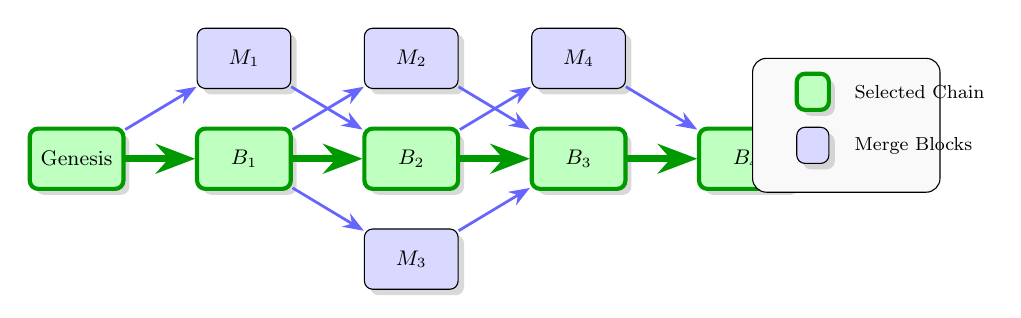
\begin{tikzpicture}[
    block/.style={rectangle, draw, fill=blue!15, minimum width=1.4cm, minimum height=0.9cm, rounded corners=3pt, font=\small, drop shadow={opacity=0.3}},
    selected/.style={rectangle, draw=green!60!black, fill=green!25, minimum width=1.4cm, minimum height=0.9cm, rounded corners=3pt, line width=1.5pt, font=\small, drop shadow={opacity=0.3}},
    arrow/.style={->, >=Stealth, thick},
    scale=0.85, transform shape
]
    % Genesis
    \node[selected] (g) at (0,0) {Genesis};
    
    % Layer 1
    \node[selected] (b1) at (2.5,0) {$B_1$};
    \node[block] (m1) at (2.5,1.5) {$M_1$};
    
    % Layer 2
    \node[selected] (b2) at (5,0) {$B_2$};
    \node[block] (m2) at (5,1.5) {$M_2$};
    \node[block] (m3) at (5,-1.5) {$M_3$};
    
    % Layer 3
    \node[selected] (b3) at (7.5,0) {$B_3$};
    \node[block] (m4) at (7.5,1.5) {$M_4$};
    
    % Layer 4
    \node[selected] (b4) at (10,0) {$B_4$};
    
    % Arrows - Selected chain (thick green)
    \draw[arrow, line width=2.5pt, green!60!black] (g) -- (b1);
    \draw[arrow, line width=2.5pt, green!60!black] (b1) -- (b2);
    \draw[arrow, line width=2.5pt, green!60!black] (b2) -- (b3);
    \draw[arrow, line width=2.5pt, green!60!black] (b3) -- (b4);
    
    % Arrows - Merge blocks (thinner, blue-gray)
    \draw[arrow, blue!60, line width=1pt] (g) -- (m1);
    \draw[arrow, blue!60, line width=1pt] (m1) -- (b2);
    \draw[arrow, blue!60, line width=1pt] (b1) -- (m2);
    \draw[arrow, blue!60, line width=1pt] (m2) -- (b3);
    \draw[arrow, blue!60, line width=1pt] (b1) -- (m3);
    \draw[arrow, blue!60, line width=1pt] (m3) -- (b3);
    \draw[arrow, blue!60, line width=1pt] (b2) -- (m4);
    \draw[arrow, blue!60, line width=1pt] (m4) -- (b4);
    
    % Legend box
    \begin{scope}[shift={(11.5,0.5)}]
        \node[draw, rounded corners=5pt, fill=gray!5, minimum width=2.8cm, minimum height=2cm] at (0,0) {};
        \node[selected, scale=0.6, minimum width=0.8cm] at (-0.5,0.5) {};
        \node[right, font=\footnotesize] at (0,0.5) {Selected Chain};
        \node[block, scale=0.6, minimum width=0.8cm] at (-0.5,-0.3) {};
        \node[right, font=\footnotesize] at (0,-0.3) {Merge Blocks};
    \end{scope}
\end{tikzpicture}
\caption{Kaspa BlockDAG Structure. The green blocks form the selected parent chain (backbone), while blue blocks are merge-set blocks that get ordered relative to the selected chain.}
\label{fig:blockdag}
\end{figure}

Recent proposals for Kaspa aimed to address two key issues:

\textbf{Sequencing Commitment (KIP-15):} How to commit each block to the global canonical order of all transactions up to that point, so that Layer-2 (L2) systems can trustlessly follow the exact L1 transaction sequence~\cite{kip15}. KIP-15 proposed adding a chained commitment in each block header that hashes together the previous commitment and the Merkle root of the current block's accepted transactions: $\text{SC}_n = H(\text{SC}_{n-1} \parallel \text{OrderRoot}_n)$. While straightforward, a purely linear commitment implies that to prove a transaction from many blocks ago, one might need to traverse or reveal a long chain of commitments---a verification cost linear in the distance between blocks, which is prohibitive for L2 verification if the distance is large.

\textbf{Logarithmic Inclusion Proofs (KIP-6):} How to enable compact proofs (of size $\bigO(\log N)$) that a given transaction was included in the ledger by a certain block, without requiring a client to download or trust the entire chain history~\cite{kip6}. KIP-6 recognized that naive proofs of inclusion in Kaspa (or any chain) could be linear in the distance from the block to be verified. The proposal aimed to use an auxiliary data structure or protocol so that one need not traverse every block, reminiscent of the FlyClient approach for light clients.

Each of these alone solves part of the problem, but implementing them separately would mean maintaining two parallel commitment structures: one for ordering and one for efficient proofs. As noted in recent research on Merkle structures~\cite{merklebelt}, a linear hash chain is essentially a degenerate ``mountain range'' with exactly one peak that grows linearly---maximally unbalanced and far from succinct, forcing proofs to be as long as the list itself.

In this paper, we propose a unified solution that achieves both goals simultaneously by leveraging a data structure called a \textbf{Merkle Mountain Range (MMR)} as a historical accumulator of block commitments. MMRs were first popularized by Todd for Bitcoin-like systems~\cite{todd2012mmr} as a way to commit to ever-growing data with the ability to produce logarithmic-sized proofs of membership. By replacing the linear sequencing commitment with an MMR commitment, we dramatically improve proof efficiency from $\bigO(N)$ to $\bigO(\log N)$.

\subsection{Our Contributions}

Our approach, which we call the \emph{MMR-based Sequencing Commitment}, integrates with Kaspa's consensus as follows:
\begin{itemize}
    \item Every block contains a commitment to the set of transactions it accepts (in canonical order) via an \code{order\_root} (replacing the legacy accepted-ID Merkle root in the header).
    \item Every block also carries an \code{mmr\_root} and \code{mmr\_size}, which accumulate all prior blocks' commitments (leaves) in an append-only Merkle Mountain Range. The MMR acts as a logarithmic-size historical log of the sequence commitments.
    \item The combination allows any transaction's inclusion position to be proven with two linked proofs: an intra-block Merkle proof to show the transaction is in a block's accepted list, and an MMR proof to show that block's leaf is in the MMR as of some recent block. The latter is of logarithmic size in the number of blocks spanned.
\end{itemize}

This design effectively provides \textbf{everlasting cryptographic receipts} for transactions in Kaspa: a light client or an L2 contract can verify that a transaction was confirmed in block $B$ and at position $k$ in the global order by checking a short proof against a recent block header's MMR root. The proof size and verification cost grow only logarithmically with the age of the transaction, rather than linearly as in a simple chained commitment scheme.

In particular, our contributions and findings include:
\begin{enumerate}
    \item \textbf{Unified Commitment Scheme:} We design a consensus change for Kaspa that introduces two new fields, \code{order\_root} and \code{mmr\_root} (along with a size indicator), into each block header. The \code{order\_root} commits to the block's local transaction order (as per KIP-15), and the \code{mmr\_root} cumulatively includes an entry for every block on the selected chain. This single scheme intertwines KIP-15 and KIP-6 into one mechanism.
    
    \item \textbf{Formalization of Canonical Order in a DAG:} We clarify how the canonical transaction order is derived in Kaspa's DAG context, defining $\TxList(B)$ as the exact sequence of accepted transaction IDs determined by consensus, ensuring determinism across all nodes.
    
    \item \textbf{MMR Integration and Algorithms:} We describe how MMR leaves are computed and appended using only data available at block validation time (avoiding circular dependencies). We specify the append algorithm and calculation of the MMR root using deterministic bagging of peaks with fixed domain prefixes.
    
    \item \textbf{Compact Inclusion Proofs:} We define the structure of MMR inclusion proofs and show that a smart contract or light client can verify a transaction's inclusion in Kaspa's history by: (1) checking the transaction hash against the block's \code{order\_root} via intra-block Merkle proof, and (2) checking the block's leaf against the known \code{mmr\_root} via the MMR proof. Both proofs are logarithmic in size.
    
    \item \textbf{Quantitative Analysis:} We demonstrate that verifying a transaction from 100,000 blocks ago requires only $\sim$17 hash operations in our scheme versus 100,000 sequential hashes in a traditional chain commitment---a 99.98\% reduction in verification cost.
\end{enumerate}

\subsection{Paper Organization}

The rest of this paper is organized as follows. Section~\ref{sec:background} provides background on Kaspa's DAG and the need for canonical ordering and efficient proofs, including an introduction to Merkle Mountain Ranges. Section~\ref{sec:design} describes the design of the MMR-based sequencing commitment in detail. Section~\ref{sec:reorg} addresses how we handle challenges like block reorganization and pruning. Section~\ref{sec:proofs} discusses the proof construction and verification. Section~\ref{sec:applications} explores important use cases and benefits. Section~\ref{sec:overhead} analyzes the overhead and performance. Section~\ref{sec:comparison} compares our approach with the separate KIP-15 and KIP-6 schemes. Implementation considerations are given in Section~\ref{sec:implementation}. Finally, Section~\ref{sec:conclusion} concludes with a summary and implications for future blockchain designs.

%==============================================================================
% SECTION 2: BACKGROUND
%==============================================================================
\section{Background and Motivation}
\label{sec:background}

\subsection{Blockchain Transaction Ordering and Proofs}

In a conventional blockchain (single chain of blocks), establishing the order of transactions and providing proofs of inclusion is straightforward: all blocks form a linear sequence, and within each block a Merkle tree commits to the transactions. A client given a block header (with the Merkle root) and a transaction plus a Merkle branch can verify that transaction was included in that block. To trust that this block is part of the canonical chain, the client must also verify the chain of block hashes (or a proof-of-work difficulty sequence) from a known checkpoint up to that block.

Verifying a transaction from $N$ blocks ago thus typically requires $\bigO(\log M)$ work for the Merkle proof (where $M$ is the number of transactions in that block) plus $\bigO(N)$ work to verify the block's inclusion in the chain (unless some accumulator of block headers is used).

Kaspa's blockDAG architecture complicates this in two ways:
\begin{enumerate}
    \item There isn't a single chain of blocks---blocks can be created concurrently and reference multiple parents. Kaspa's consensus (GHOSTDAG) assigns a partial order to blocks and designates one parent of each block as the \emph{selected parent}.
    \item Because blocks are not strictly sequential, defining a canonical order of transactions is non-trivial. Kaspa's consensus does produce a deterministic ordering of blocks, but this order must be agreed upon and consistent across all nodes.
\end{enumerate}

The motivation for having an explicit commitment to transaction ordering is largely driven by Layer-2 scalability solutions (like rollups or payment channels) and cross-chain bridges. These systems need to verify L1 events with minimal trust. Without a specialized commitment, verifying an event from an old block might require linear work in the number of blocks since then---impractical on-chain or for light clients.

\subsection{Merkle Mountain Ranges (MMR)}

Our solution employs Merkle Mountain Ranges (MMRs) as the core data structure to achieve an efficient historical commitment~\cite{herodotus}. An MMR is a type of append-only Merkle tree structure especially suited for sequentially growing datasets.

\begin{definition}[Merkle Mountain Range]
An MMR is defined over an indexed sequence of leaves (data items) numbered from $0$ onward. It can be thought of as a forest of perfect binary trees (``mountains'') whose sizes correspond to the binary decomposition of the leaf count. For $N$ leaves, if $N = \sum_{i} 2^{b_i}$ in binary, then the MMR consists of trees of sizes $2^{b_i}$.
\end{definition}

\begin{figure}[htbp]
\centering
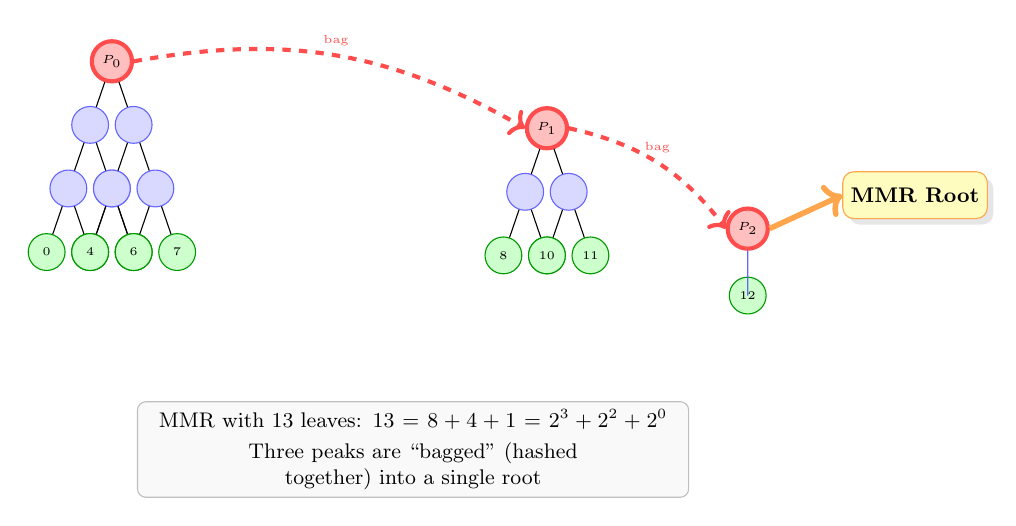
\begin{tikzpicture}[
    node/.style={circle, draw=blue!60, fill=blue!15, minimum size=0.55cm, font=\tiny, inner sep=1pt},
    leaf/.style={circle, draw=green!60!black, fill=green!20, minimum size=0.55cm, font=\tiny, inner sep=1pt},
    peak/.style={circle, draw=red!70, fill=red!25, minimum size=0.6cm, font=\tiny\bfseries, line width=1.5pt, inner sep=1pt},
    level distance=0.95cm,
    sibling distance=0.65cm,
    scale=0.85, transform shape
]
    % Mountain 1 (size 8) - positioned manually for better control
    \node[peak] (r1) at (3,3) {$P_0$}
        child {node[node] {}
            child {node[node] {}
                child {node[leaf] {0}}
                child {node[leaf] {1}}
            }
            child {node[node] {}
                child {node[leaf] {2}}
                child {node[leaf] {3}}
            }
        }
        child {node[node] {}
            child {node[node] {}
                child {node[leaf] {4}}
                child {node[leaf] {5}}
            }
            child {node[node] {}
                child {node[leaf] {6}}
                child {node[leaf] {7}}
            }
        };
    
    % Mountain 2 (size 4)
    \node[peak] (r2) at (9.5,2) {$P_1$}
        child {node[node] {}
            child {node[leaf] {8}}
            child {node[leaf] {9}}
        }
        child {node[node] {}
            child {node[leaf] {10}}
            child {node[leaf] {11}}
        };
    
    % Mountain 3 (size 1)
    \node[peak] (r3) at (12.5,0.5) {$P_2$};
    \node[leaf] at (12.5,-0.5) {12};
    \draw[blue!60] (r3) -- (12.5,-0.5);
    
    % Bagging arrows with clearer styling
    \draw[->, line width=1.5pt, dashed, red!70] (r1.east) to[bend left=20] node[above, font=\tiny, red!70] {bag} (r2.west);
    \draw[->, line width=1.5pt, dashed, red!70] (r2.east) to[bend left=20] node[above, font=\tiny, red!70] {bag} (r3.west);
    
    % Final root box
    \node[draw=orange!70, fill=yellow!25, rounded corners=4pt, font=\small\bfseries, minimum width=1.8cm, minimum height=0.7cm, drop shadow={opacity=0.2}] (root) at (15,1) {MMR Root};
    \draw[->, line width=2pt, orange!70] (r3.east) -- (root.west);
    
    % Annotation box at bottom
    \node[draw=gray!50, fill=gray!5, rounded corners=3pt, font=\small, align=center, text width=8cm] at (7.5,-2.8) {
        MMR with 13 leaves: $13 = 8 + 4 + 1 = 2^3 + 2^2 + 2^0$\\[2pt]
        Three peaks are ``bagged'' (hashed together) into a single root
    };
\end{tikzpicture}
\caption{Merkle Mountain Range structure with 13 leaves. The structure consists of three ``mountains'' (perfect binary trees) corresponding to the binary representation $13_{10} = 1101_2$. Peaks $P_0$, $P_1$, $P_2$ are hashed together (bagged) to produce the final MMR root.}
\label{fig:mmr-structure}
\end{figure}

Key properties of MMRs that make them attractive for blockchain history accumulators include:

\begin{enumerate}
    \item \textbf{Append-Only and Efficient Updates:} Adding a new leaf to an MMR takes $\bigO(\log N)$ hashing work. The MMR doesn't require a fixed tree size or re-balancing; it naturally accommodates continuous growth.
    
    \item \textbf{Succinct Proofs:} To prove that a given leaf is included in the MMR, one provides a proof consisting of the leaf's sibling nodes up through the tree and the list of peaks. The size of this proof is at most $\bigO(\log N)$ hashes.
    
    \item \textbf{Immutability and Unique Representation:} The structure of the MMR is fully determined by the number of leaves. For a given sequence of $N$ items, the MMR will always produce the same set of peak hashes and the same root.
    
    \item \textbf{Inclusion of Historical Data:} Unlike a simple moving hash (like a chain of hashes), the MMR's peaks collectively incorporate all past leaves. Even older blocks far down the ``mountain range'' are still cryptographically linked into the latest root.
\end{enumerate}

\textbf{Appending Algorithm:} When a new leaf is added to the MMR, it is appended as a new tree of size 1 (a new peak). If the previously last tree (peak) also had size 1, then the two single leaves are merged to form a tree of size 2. This might in turn merge with a next peak of size 2 to form a size 4 tree, and so on. In general, the rule is: upon adding the $(n+1)$-th leaf, look at the binary representation of $n$. Each trailing 1 in $n$ indicates a peak that will merge with the new leaf (or intermediate result of merges) to form a larger peak. This is equivalent to ``carrying'' in binary addition.

\textbf{Example:} If $n = 7$ (binary $111$, with trailing ones), there were peaks of sizes 1, 2, 4. A new leaf causes the size-1 peak and new leaf to merge (size 2), then that merges with the existing size-2 peak to form size 4, then that merges with the existing size-4 peak to form a size-8 peak. Now for $n+1 = 8$ ($1000_2$), there is just one peak of size 8. If $n = 4$ (binary $100$, already a perfect tree of size 4 with one peak), adding a leaf results in $n+1 = 5$ ($101_2$) which will have two peaks: the old size-4 peak remains and the new leaf stands alone as a size-1 peak.

\textbf{MMR vs. Linear Chain:} A linear hash chain (each block contains the hash of the previous block) is essentially an extreme case of a Merkle structure---a degenerate ``mountain range'' with exactly one peak that grows linearly. The proof that a given block was in the chain of length $N$ is of length $N$ (one would have to show each link). As noted in recent research~\cite{merklebelt}, the linear chain is maximally unbalanced and far from succinct; it forces proofs to be as long as the list itself. In contrast, an MMR is balanced and yields succinct proofs (logarithmic in $N$).

\subsection{Kaspa DAG, Selected Chain, and Canonical Transaction Order}

\textbf{Kaspa's BlockDAG:} Kaspa is a blockDAG where blocks reference multiple parents. This yields high throughput (e.g., 10 blocks per second) but requires a rule to determine a total ordering. Kaspa's consensus (GHOSTDAG) assigns each block a \emph{blue score} and orders blocks by essentially sorting by blue score and hash. For each new block, one of its parents is labeled the \emph{selected parent} (SP)---usually the one with the highest blue score. The set of blocks not on the selected parent chain but referenced by the new block are called the block's \emph{mergeset}.

\textbf{Accepted Transactions:} When a new block arrives, not all transactions in its mergeset are necessarily accepted. If two parallel blocks contain a conflicting transaction (double spend), only the transactions from the block that is ``preferred'' by GHOSTDAG (the blue set) will be accepted. However, all non-conflicting transactions from all blocks will be included in the ledger's UTXO state.

\begin{figure}[htbp]
\centering
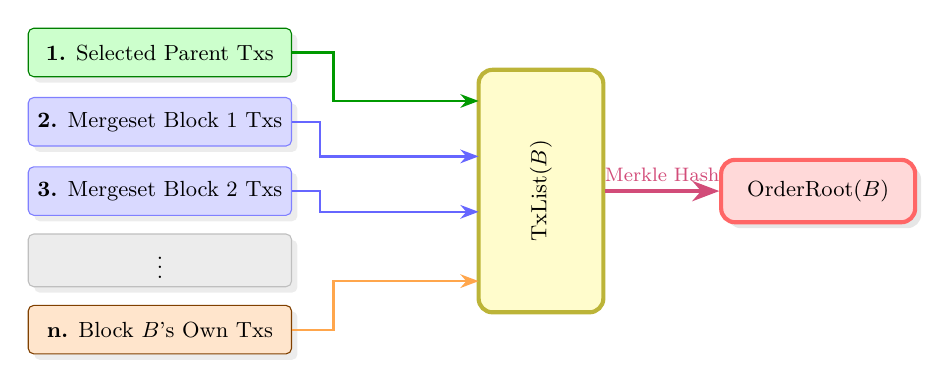
\begin{tikzpicture}[
    box/.style={rectangle, draw, rounded corners=2pt, minimum width=3.8cm, minimum height=0.7cm, font=\small, drop shadow={opacity=0.15}},
    arrow/.style={->, >=Stealth, thick},
    scale=0.88, transform shape
]
    % Input boxes with numbered order
    \node[box, fill=green!20, draw=green!50!black] (sp) at (0,4) {\textbf{1.} Selected Parent Txs};
    \node[box, fill=blue!15, draw=blue!50] (m1) at (0,3) {\textbf{2.} Mergeset Block 1 Txs};
    \node[box, fill=blue!15, draw=blue!50] (m2) at (0,2) {\textbf{3.} Mergeset Block 2 Txs};
    \node[box, fill=gray!15, draw=gray!50] (dots) at (0,1) {$\vdots$};
    \node[box, fill=orange!20, draw=orange!50!black] (own) at (0,0) {\textbf{n.} Block $B$'s Own Txs};
    
    % TxList container
    \node[draw=yellow!70!black, rounded corners=5pt, fill=yellow!20, minimum width=1.8cm, minimum height=3.5cm, line width=1.5pt] (txlist) at (5.5,2) {};
    \node[font=\small\bfseries, rotate=90] at (5.5,2) {$\TxList(B)$};
    
    % Arrows to TxList
    \draw[arrow, green!60!black] (sp.east) -- ++(0.6,0) |- (4.6,3.3);
    \draw[arrow, blue!60] (m1.east) -- ++(0.4,0) |- (4.6,2.5);
    \draw[arrow, blue!60] (m2.east) -- ++(0.4,0) |- (4.6,1.7);
    \draw[arrow, orange!70] (own.east) -- ++(0.6,0) |- (4.6,0.7);
    
    % OrderRoot
    \node[draw=red!60, rounded corners=5pt, fill=red!15, minimum width=2.8cm, minimum height=0.9cm, line width=1.5pt, font=\small\bfseries, drop shadow={opacity=0.2}] (orderroot) at (9.5,2) {$\OrderRoot(B)$};
    
    % Arrow with label
    \draw[arrow, line width=1.5pt, purple!70] (txlist.east) -- node[above, font=\footnotesize, text=purple!70] {Merkle Hash} (orderroot.west);
\end{tikzpicture}
\caption{Construction of the canonical transaction list ($\TxList$) and $\OrderRoot$ for block $B$. Transactions are ordered deterministically: selected parent first, then mergeset blocks in consensus order, finally block $B$'s own transactions.}
\label{fig:txlist-construction}
\end{figure}

Kaspa's node implementation computes, for each block $B$, the set of \emph{accepted transaction IDs}---essentially the union of the transactions in the block's selected parent and those in the block's remaining mergeset (excluding conflicts), in a deterministic order. By walking through the DAG following the selected chain and at each block outputting its accepted transaction list, one obtains a single global sequence of transactions. This global sequence is what an L2 system would interpret as the history of L1 transactions.

\textbf{Detailed Example:} Consider a simple DAG scenario for illustration. Suppose block $B_1$ is the genesis, and two blocks $B_2$ and $B_3$ are mined concurrently on $B_1$. Then a block $B_4$ comes selecting $B_2$ as its parent, and another $B_5$ selecting $B_3$, and finally $B_6$ selecting $B_4$ and also referencing $B_5$:
\begin{center}
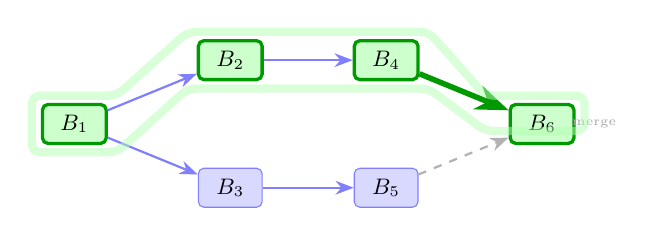
\begin{tikzpicture}[
    block/.style={rectangle, draw=blue!50, fill=blue!15, minimum width=0.9cm, minimum height=0.55cm, font=\small, rounded corners=2pt},
    selected/.style={rectangle, draw=green!60!black, fill=green!20, minimum width=0.9cm, minimum height=0.55cm, font=\small, line width=1.2pt, rounded corners=2pt},
    arrow/.style={->, >=Stealth, thick},
    scale=0.9, transform shape
]
    \node[selected] (b1) at (0,0) {$B_1$};
    \node[selected] (b2) at (2.2,0.9) {$B_2$};
    \node[block] (b3) at (2.2,-0.9) {$B_3$};
    \node[selected] (b4) at (4.4,0.9) {$B_4$};
    \node[block] (b5) at (4.4,-0.9) {$B_5$};
    \node[selected] (b6) at (6.6,0) {$B_6$};
    
    \draw[arrow, blue!50] (b1) -- (b2);
    \draw[arrow, blue!50] (b1) -- (b3);
    \draw[arrow, blue!50] (b2) -- (b4);
    \draw[arrow, blue!50] (b3) -- (b5);
    \draw[arrow, line width=2pt, green!60!black] (b4) -- (b6);
    \draw[arrow, dashed, gray!60] (b5) -- (b6);
    
    \node[font=\tiny, text=gray!70, right] at (6.9,0) {merge};
    
    % Selected chain highlight
    \draw[line width=3pt, green!30, opacity=0.5, rounded corners=3pt] 
        (-0.6,-0.4) -- (0.6,-0.4) -- (1.6,0.5) -- (2.8,0.5) -- (3.8,0.5) -- (5,0.5) -- (5.8,-0.1) -- (7.2,-0.1) -- (7.2,0.4) -- (5.8,0.4) -- (5,1.3) -- (3.8,1.3) -- (2.8,1.3) -- (1.6,1.3) -- (0.6,0.4) -- (-0.6,0.4) -- cycle;
\end{tikzpicture}
\end{center}

Here the selected parent chain is: $B_1 \to B_2 \to B_4 \to B_6$ (green blocks). The canonical transaction sequence up to $B_6$ would then be:
\begin{enumerate}[noitemsep]
    \item $\TxList(B_1)$: all transactions from genesis
    \item $\TxList(B_2)$: transactions from $B_2$
    \item Transactions from $B_3$ not already included (merged when $B_4$ or $B_6$ processes its mergeset)
    \item $\TxList(B_4)$: transactions from $B_4$
    \item Transactions from $B_5$ not already included (merged when $B_6$ is processed)
    \item $\TxList(B_6)$: transactions from $B_6$
\end{enumerate}
This results in one total order of all accepted transactions up to block $B_6$. If two transactions conflict (double-spend), Kaspa's consensus ensures only one will be accepted---generally the one appearing in the earlier position in the canonical order.

KIP-15's originally suggested mechanism was to maintain a running hash chain: $SC_n = H(SC_{n-1} \parallel \OrderRoot(B_n))$. While this achieves commitment to the sequence, it inherits a major limitation: verifying that a given old block's transactions are in the chain up to some later point requires iterating through each block's hash link in between (linear complexity). Our approach replaces this linear chain of commitments with the MMR accumulator, which breaks the sequential dependency and allows skip-ahead verification.

%==============================================================================
% SECTION 3: DESIGN
%==============================================================================
\section{MMR-Based Sequencing Commitment Design}
\label{sec:design}

In this section, we present the detailed design of the MMR-based sequencing commitment. We describe the modifications to the Kaspa block header, define how the MMR is computed and updated with each new block, and specify the consensus rules for validation.

\subsection{Block Header Modifications}

We extend the Kaspa block header with two new fields and modify one existing field:

\begin{table}[htbp]
\centering
\caption{Block Header Field Modifications}
\label{tab:header-fields}
\begin{tabular}{@{}llp{7cm}@{}}
\toprule
\textbf{Field} & \textbf{Size} & \textbf{Description} \\
\midrule
\code{order\_root} & 32 bytes & Merkle root of accepted transaction IDs for this block, representing the set of transactions (in canonical order) confirmed by this block's addition to the ledger \\
\code{mmr\_root} & 32 bytes & MMR root hash after inserting this block's leaf, serving as a cryptographic commitment to the entire history of transaction order \\
\code{mmr\_size} & 8 bytes & Total number of leaves in the MMR after adding this block \\
\midrule
\multicolumn{3}{l}{\textit{Removed field:}} \\
\code{accepted\_id\_merkle\_root} & 32 bytes & (Replaced by \code{order\_root}) \\
\midrule
\textbf{Net Change} & \textbf{+40 bytes} & ($2 \times 32 + 8 - 32 = 40$ bytes per header) \\
\bottomrule
\end{tabular}
\end{table}

At 10 blocks/sec, the net increase is $\sim$34.6 MB per day, which is negligible overhead for network transmission (roughly 0.08\% of typical block data throughput).

\subsection{Canonical Order and OrderRoot Computation}

\begin{definition}[Canonical Transaction List]
For each block $B$, we define an ordered list of transaction IDs, denoted $\TxList(B)$, which is the sequence of all accepted transactions that are considered to ``happen at'' block $B$ in the global order. This list is constructed from the block's selected parent and mergeset in the consensus processing.
\end{definition}

Suppose block $B$ has selected parent $P_{\text{sel}}$ and a set of merge parents $\{M_1, M_2, \dots, M_k\}$. The UTXO validation algorithm in Kaspa will process:
\begin{enumerate}
    \item The coinbase transaction of $P_{\text{sel}}$ (if not already included earlier)
    \item The remaining transactions of $P_{\text{sel}}$, in their original order
    \item The transactions from each merge block $M_i$ in a deterministic order
    \item Transactions in $B$ itself
\end{enumerate}

We define:
\begin{equation}
\OrderRoot(B) := \MerkleRoot(\TxList(B))
\end{equation}

\textbf{Determinism and Security:} Because all honest nodes will derive the same $\TxList$ for $B$, the $\OrderRoot$ is an objective, deterministic value. If a malicious miner tried to put a different $\OrderRoot$ in the header that doesn't match the actual transactions, consensus validation will catch it.

\subsection{MMR Leaf and Internal Hashing Scheme}

For each block $B$ that lies on the selected parent chain, we create an MMR leaf node:
\begin{equation}
L(B) = \Hleaf(h_{P_{\text{sel}}(B)} \parallel \OrderRoot(B))
\end{equation}
where $h_{P_{\text{sel}}(B)}$ is the hash of $B$'s selected parent block header, and $\Hleaf$ is a hash function instance domain-separated for leaf hashing.

\textbf{Rationale for leaf contents:}
\begin{itemize}
    \item We include the selected parent's hash to anchor this leaf in the chain of blocks. This ensures that if a block is reordered or placed under a different parent, its leaf hash would change.
    \item We include the $\OrderRoot$ to commit to the transaction content.
    \item We do \emph{not} include the block's own hash in the leaf to avoid a circular dependency: the block's hash itself is computed from the header fields, which include the MMR root.
\end{itemize}

\begin{figure}[htbp]
\centering
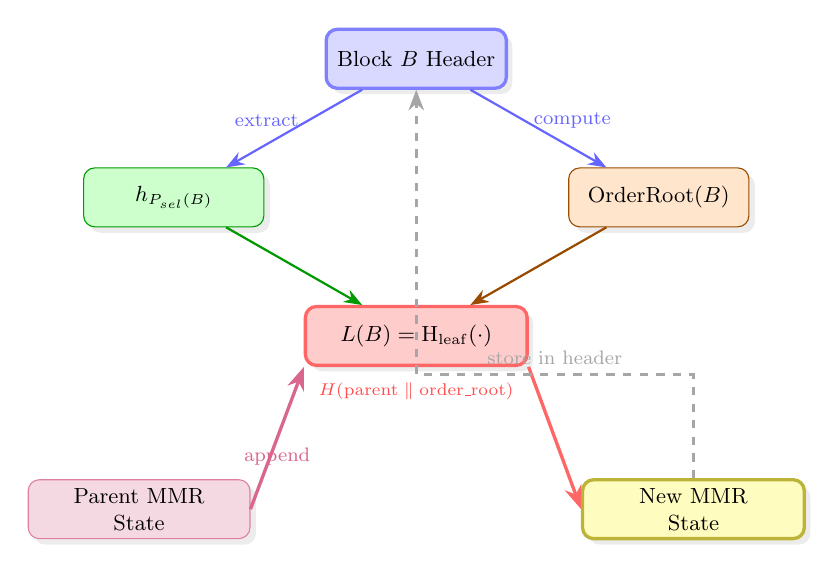
\begin{tikzpicture}[
    box/.style={rectangle, draw, rounded corners=4pt, minimum width=2.6cm, minimum height=0.85cm, font=\small, drop shadow={opacity=0.15}},
    arrow/.style={->, >=Stealth, thick},
    scale=0.88, transform shape
]
    % Block B Header (top)
    \node[box, fill=blue!15, draw=blue!50, line width=1.2pt] (header) at (0,3.5) {Block $B$ Header};
    
    % Parent Hash (left)
    \node[box, fill=green!20, draw=green!60!black] (parent) at (-3.5,1.5) {$h_{P_{sel}(B)}$};
    
    % OrderRoot (right)
    \node[box, fill=orange!20, draw=orange!60!black] (order) at (3.5,1.5) {$\OrderRoot(B)$};
    
    % Leaf hash (center)
    \node[box, fill=red!20, draw=red!60, line width=1.2pt, minimum width=3.2cm] (leaf) at (0,-0.5) {$L(B) = \Hleaf(\cdot)$};
    
    % MMR State boxes
    \node[box, fill=purple!15, draw=purple!50, minimum width=3.2cm, align=center] (mmrstate) at (-4,-3) {Parent MMR\\State};
    
    \node[box, fill=yellow!25, draw=yellow!70!black, minimum width=3.2cm, align=center, line width=1.2pt] (newmmr) at (4,-3) {New MMR\\State};
    
    % Arrows with labels
    \draw[arrow, blue!60] (header) -- node[left, font=\footnotesize, pos=0.4] {extract} (parent);
    \draw[arrow, blue!60] (header) -- node[right, font=\footnotesize, pos=0.4] {compute} (order);
    \draw[arrow, green!60!black] (parent) -- (leaf);
    \draw[arrow, orange!60!black] (order) -- (leaf);
    \draw[arrow, purple!60, line width=1.2pt] (mmrstate.east) -- node[below, font=\footnotesize, text=purple!60] {append} (leaf.south west);
    \draw[arrow, red!60, line width=1.2pt] (leaf.south east) -- (newmmr.west);
    
    % Feedback loop (dashed)
    \draw[arrow, dashed, gray!70, line width=1pt] (newmmr.north) -- ++(0,1.5) -| node[pos=0.25, above, font=\footnotesize, text=gray!70] {store in header} (header.south);
    
    % Hash symbol at leaf
    \node[font=\scriptsize, text=red!70] at (0,-1.3) {$H(\text{parent} \parallel \text{order\_root})$};
\end{tikzpicture}
\caption{MMR leaf computation and state update flow. The leaf is computed from parent hash and $\OrderRoot$, then appended to the parent's MMR state to produce the new MMR root stored in the block header.}
\label{fig:mmr-computation}
\end{figure}

\textbf{MMR Structure Maintenance:} The MMR is maintained as follows. Let $S(n)$ denote the state of the MMR after processing $n$ leaves. When a new leaf arrives:
\begin{enumerate}
    \item We initially consider the new leaf as a new peak (a tree of size 1)
    \item As long as we have two peaks of equal size, we merge them (like adding binary numbers)
    \item The number of merges equals the number of trailing 1 bits in the old size
\end{enumerate}

\textbf{Internal Node Hashing:} When two peaks are merged, we use a domain-separated hash:
\begin{equation}
\text{merged} = \Hnode(\text{left\_peak} \parallel \text{right\_peak})
\end{equation}

\textbf{Peak Bagging to Root:} After processing the new leaf and merging as needed, we compute the final MMR root by hashing all peaks together (``bagging the peaks''):
\begin{align}
\text{bag}_0 &= p_0 \\
\text{bag}_{i} &= \Hbag(\text{bag}_{i-1} \parallel p_i) \quad \text{for } i = 1, \ldots, k-1 \\
\text{mmr\_root} &= \Hroot(\text{bag}_{k-1} \parallel \text{encode}_{64}(\text{mmr\_size}))
\end{align}

Including the size in the final hash ensures that different sequences of leaves cannot produce the same root. The order of peaks and the hashing procedure must be canonical and agreed upon in consensus. In our design, peaks are ordered from smallest-index (leftmost, corresponding to largest tree) to largest-index (rightmost, possibly a small tree) and hashed in that sequence.

\begin{algorithm}[htbp]
\caption{MMR Append Operation}
\label{alg:mmr-append}
\begin{algorithmic}[1]
\Require Current MMR state (peaks list, size), new leaf hash
\Ensure Updated MMR state, new root
\Function{Append}{state, new\_leaf}
    \State new\_size $\gets$ state.size $+ 1$
    \State current\_hash $\gets$ new\_leaf
    \State new\_peaks $\gets$ copy(state.peaks)
    \State count $\gets$ \Call{TrailingOnes}{state.size}
    \Comment{Number of trailing 1-bits in binary representation}
    \For{$i \gets 1$ to count}
        \State left\_peak $\gets$ new\_peaks.pop()
        \State current\_hash $\gets \Hnode(\text{left\_peak} \parallel \text{current\_hash})$
    \EndFor
    \State new\_peaks.append(current\_hash)
    \State bag $\gets$ new\_peaks[0]
    \For{$i \gets 1$ to new\_peaks.length $- 1$}
        \State bag $\gets \Hbag(\text{bag} \parallel \text{new\_peaks}[i])$
    \EndFor
    \State mmr\_root $\gets \Hroot(\text{bag} \parallel \text{encode}_{64}(\text{new\_size}))$
    \State \Return (MmrState\{peaks: new\_peaks, size: new\_size\}, mmr\_root)
\EndFunction
\end{algorithmic}
\end{algorithm}

The \textsc{TrailingOnes} function returns the number of consecutive 1 bits in the binary representation starting from the least significant bit. For example, $\textsc{TrailingOnes}(7) = 3$ (binary $111$) and $\textsc{TrailingOnes}(4) = 0$ (binary $100$). This achieves $\bigO(1)$ amortized time per append with a small constant factor for the merging.

\subsection{Consensus Validation Rules}

When processing block $B$, nodes perform the following validations:

\begin{algorithm}[htbp]
\caption{Block Validation with MMR Commitments}
\label{alg:validation}
\begin{algorithmic}[1]
\Require Block $B$ with header fields, Parent block $P$
\Ensure Block validity

\State \textbf{Step 1: Order-Root Verification}
\State $\text{expected\_order\_root} \gets \MerkleRoot(\text{accepted\_tx\_ids of } B)$
\If{$\text{expected\_order\_root} \neq B.\text{order\_root}$}
    \State \Return \textsc{BadOrderRoot}
\EndIf

\State \textbf{Step 2: MMR Leaf Computation}
\State $\text{leaf}_B \gets \Hleaf(P.\text{hash} \parallel B.\text{order\_root})$

\State \textbf{Step 3: MMR Append Computation}
\State old\_size $\gets P.\text{mmr\_size}$
\State new\_size $\gets$ old\_size $+ 1$
\State peaks $\gets P.\text{mmr\_peaks}$
\State current $\gets \text{leaf}_B$
\While{old\_size has trailing 1 bit}
    \State left\_peak $\gets$ peaks.pop()
    \State current $\gets \Hnode(\text{left\_peak} \parallel \text{current})$
    \State old\_size $\gets$ old\_size $\gg 1$
\EndWhile
\State peaks.push(current)

\State \textbf{Step 4: Compute Expected MMR Root}
\State bag $\gets$ peaks[0]
\For{$i \gets 1$ to peaks.length $- 1$}
    \State bag $\gets \Hbag(\text{bag} \parallel \text{peaks}[i])$
\EndFor
\State expected\_mmr\_root $\gets \Hroot(\text{bag} \parallel \text{encode}_{64}(\text{new\_size}))$

\State \textbf{Step 5: Verification}
\If{expected\_mmr\_root $\neq B.\text{mmr\_root}$}
    \State \Return \textsc{BadMmrRoot}
\EndIf
\If{new\_size $\neq B.\text{mmr\_size}$}
    \State \Return \textsc{BadMmrSize}
\EndIf

\State \Return \textsc{Valid}
\end{algorithmic}
\end{algorithm}

The MMR verification adds a small constant amount of work per block: computing one Merkle root (for transactions) and a handful of hashes for the MMR update. On average, this is less than 2 hashes per block, and even in worst-case bursts (when block height is a power of 2 minus 1), the hashing overhead is negligible relative to mining and other validation.

%==============================================================================
% SECTION 4: REORGANIZATIONS
%==============================================================================
\section{Handling Reorganizations and Forks}
\label{sec:reorg}

One of the challenges in a blockchain (especially a DAG-based one) is handling chain reorganization (reorg) events, where the selected parent chain may change. Kaspa's GHOSTDAG can cause the selected chain to change at the virtual block if a fork is resolved in favor of a different chain of blue blocks.

\subsection{Reorg Rollback and Recompute}

In the event of a reorg:
\begin{enumerate}
    \item Let $C$ be the last common ancestor block between the old and new selected parent chain (the fork point)
    \item The old chain had leaves for blocks after $C$ that are no longer on the selected chain
    \item The new chain has a sequence of blocks from $C$ to the new tip that were not previously on the main chain
\end{enumerate}

\begin{figure}[htbp]
\centering
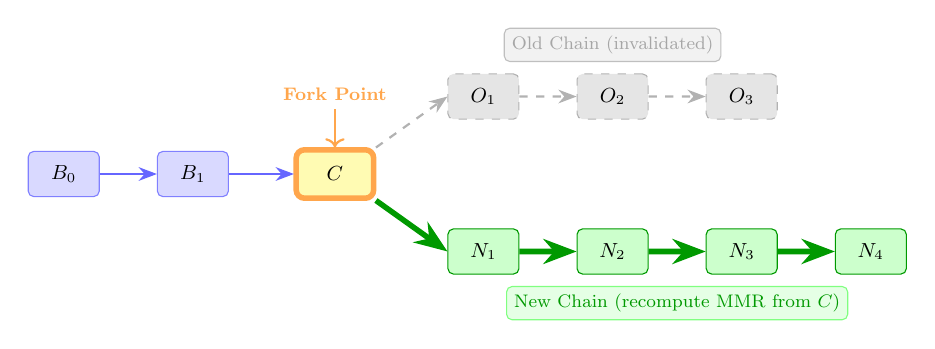
\begin{tikzpicture}[
    block/.style={rectangle, draw=blue!50, fill=blue!15, minimum width=1.1cm, minimum height=0.7cm, font=\small, rounded corners=2pt},
    oldblock/.style={rectangle, draw=gray!60, fill=gray!20, minimum width=1.1cm, minimum height=0.7cm, font=\small, rounded corners=2pt, dashed},
    newblock/.style={rectangle, draw=green!60!black, fill=green!20, minimum width=1.1cm, minimum height=0.7cm, font=\small, rounded corners=2pt},
    common/.style={rectangle, draw=orange!70, fill=yellow!30, minimum width=1.2cm, minimum height=0.75cm, font=\small\bfseries, line width=2pt, rounded corners=3pt},
    arrow/.style={->, >=Stealth, thick},
    scale=0.82, transform shape
]
    % Common chain
    \node[block] (b0) at (0,0) {$B_0$};
    \node[block] (b1) at (2,0) {$B_1$};
    \node[common] (c) at (4.2,0) {$C$};
    
    % Old chain (top, faded)
    \node[oldblock] (old1) at (6.5,1.2) {$O_1$};
    \node[oldblock] (old2) at (8.5,1.2) {$O_2$};
    \node[oldblock] (old3) at (10.5,1.2) {$O_3$};
    
    % New chain (bottom, emphasized)
    \node[newblock] (new1) at (6.5,-1.2) {$N_1$};
    \node[newblock] (new2) at (8.5,-1.2) {$N_2$};
    \node[newblock] (new3) at (10.5,-1.2) {$N_3$};
    \node[newblock] (new4) at (12.5,-1.2) {$N_4$};
    
    % Arrows - common chain
    \draw[arrow, blue!60] (b0) -- (b1);
    \draw[arrow, blue!60] (b1) -- (c);
    
    % Arrows - old chain (dashed, gray)
    \draw[arrow, dashed, gray!60, line width=0.8pt] (c.north east) -- (old1.west);
    \draw[arrow, dashed, gray!60, line width=0.8pt] (old1) -- (old2);
    \draw[arrow, dashed, gray!60, line width=0.8pt] (old2) -- (old3);
    
    % Arrows - new chain (thick, green)
    \draw[arrow, line width=2pt, green!60!black] (c.south east) -- (new1.west);
    \draw[arrow, line width=2pt, green!60!black] (new1) -- (new2);
    \draw[arrow, line width=2pt, green!60!black] (new2) -- (new3);
    \draw[arrow, line width=2pt, green!60!black] (new3) -- (new4);
    
    % Labels in boxes
    \node[draw=gray!50, fill=gray!10, rounded corners=2pt, font=\footnotesize, text=gray!70] at (8.5,2) {Old Chain (invalidated)};
    \node[draw=green!50, fill=green!10, rounded corners=2pt, font=\footnotesize, text=green!60!black] at (9.5,-2) {New Chain (recompute MMR from $C$)};
    
    % Fork point indicator
    \draw[<-, thick, orange!70] (c.north) -- ++(0,0.6) node[above, font=\footnotesize\bfseries, text=orange!70] {Fork Point};
\end{tikzpicture}
\caption{Chain reorganization handling. MMR state is retrieved from common ancestor $C$, and new chain blocks have their MMR states recomputed forward.}
\label{fig:reorg}
\end{figure}

To handle this:
\begin{itemize}
    \item We maintain the MMR state per block (peaks and size) in our store
    \item During reorg, we find $C$ (the common ancestor) and retrieve $C$'s MMR state
    \item We iterate forward from $C$ along the new selected chain, recomputing the MMR state for each block
\end{itemize}

Reorg handling is $\bigO(k)$ where $k$ is the number of blocks switched, typically small.

\subsection{MMR Node Storage (Enabling Proof Generation)}

While the peaks alone are enough for consensus validation (we just need to recompute the new root), generating an actual inclusion proof for an arbitrary past block or transaction requires access to the intermediate nodes (siblings along the path). A full node that wants to support light clients or bridges with proofs should maintain an \textbf{MMR Node Store} mapping each node position to its hash.

\textbf{Indexing Scheme:} The positions can be indexed by a single number if we linearize the MMR tree in a certain traversal. A simple scheme is:
\begin{itemize}
    \item Label the leaves with indices starting from 0
    \item Label internal nodes in the order they are created during the append process
    \item The position of a node can be derived from the leaf index and the node's height
\end{itemize}

We store each node hash keyed by its position. To produce a proof for leaf $i$, we:
\begin{enumerate}
    \item Compute the positions of each sibling on the path from that leaf to the peak
    \item Retrieve those sibling hashes from the store
    \item Also retrieve the peak hashes
\end{enumerate}
All of this is $\bigO(\log n)$ operations.

\textbf{Storage Cost:} Each leaf or internal node is one hash (32 bytes). An MMR with $n$ leaves has $< 2n$ nodes in total (similar to a full binary tree). The node store size for $n$ leaves is roughly $2n \times 32$ bytes:
\begin{itemize}
    \item After 1,000,000 leaves: $2 \times 10^6 \times 32 = 64$ MB
    \item After 300,000,000 leaves ($\sim$1 year at 10 BPS): $\sim$19.2 GB
\end{itemize}
This is within reason for a well-resourced node serving many light clients.

\textbf{Recommended Storage Practice:} For a full node at 10 BPS:
\begin{enumerate}
    \item Store all block headers permanently (few tens of GB/year)---required for consensus
    \item Maintain an MMR node store persistently ($\sim$20 GB/year) if supporting historical proofs
    \item Maintain a rolling cache of peaks for recent blocks (last day or week) for fast reorg handling. For example, 86,400 blocks for a day at 10 BPS with $\sim$20 peaks each $\approx$ 55 MB
\end{enumerate}

\subsection{Pruning and Checkpointing}

Kaspa nodes may prune old blocks, but they typically keep all headers (including the MMR fields). Thus, a pruned node can still verify a proof of inclusion for a pruned block: it has that block's header and the tip header.

A headers-only node can verify inclusion of a transaction from any block, given a correct proof. This is by design: enabling light clients to be almost as secure as full nodes for checking inclusion, without storing everything. The MMR commitment turns the whole history into a \emph{self-authenticating log}: the node can verify any historical data from an untrusted source against the known \code{mmr\_root}.

%==============================================================================
% SECTION 5: PROOFS
%==============================================================================
\section{Inclusion Proofs and Verification}
\label{sec:proofs}

A major goal of this design is to enable efficient transaction inclusion proofs that a light client or smart contract can verify.

\subsection{Proof Composition}

To prove that a transaction $tx$ was included in the Kaspa ledger, we need to provide evidence for two things:
\begin{enumerate}
    \item \textbf{Transaction-in-Block:} $tx$ is included in block $B$'s accepted transaction list at a certain index
    \item \textbf{Block-in-Ledger:} Block $B$'s commitment leaf is included in the MMR up to some known recent block $T$
\end{enumerate}

\begin{figure}[htbp]
\centering
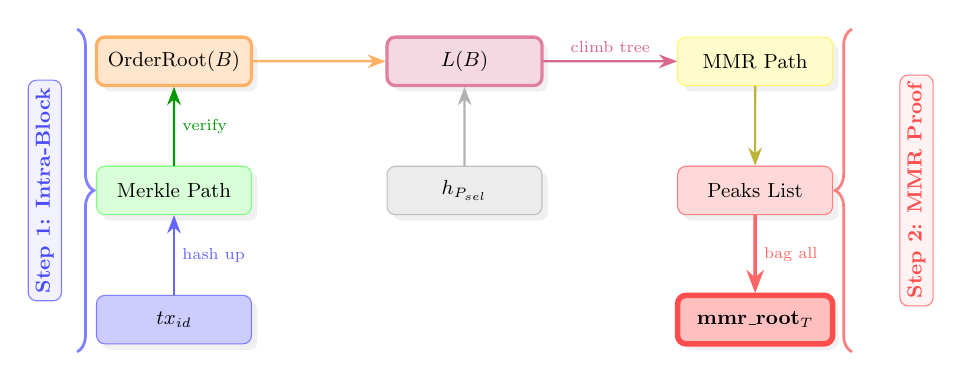
\begin{tikzpicture}[
    box/.style={rectangle, draw, rounded corners=3pt, minimum width=2.4cm, minimum height=0.75cm, font=\small, drop shadow={opacity=0.12}},
    arrow/.style={->, >=Stealth, thick},
    scale=0.82, transform shape
]
    % Step 1: Intra-Block (left column)
    \node[box, fill=blue!20, draw=blue!50] (tx) at (0,0) {$tx_{id}$};
    \node[box, fill=green!15, draw=green!50] (merkle) at (0,2) {Merkle Path};
    \node[box, fill=orange!20, draw=orange!60, line width=1.2pt] (order) at (0,4) {$\OrderRoot(B)$};
    
    % Middle column (leaf computation)
    \node[box, fill=purple!15, draw=purple!50, line width=1.2pt] (leaf) at (4.5,4) {$L(B)$};
    \node[box, fill=gray!15, draw=gray!50] (parent) at (4.5,2) {$h_{P_{sel}}$};
    
    % Step 2: MMR (right column)
    \node[box, fill=yellow!20, draw=yellow!60] (mmrpath) at (9,4) {MMR Path};
    \node[box, fill=red!15, draw=red!50] (peaks) at (9,2) {Peaks List};
    \node[box, fill=red!25, draw=red!70, line width=2pt, font=\small\bfseries] (mmrroot) at (9,0) {$\text{mmr\_root}_T$};
    
    % Arrows with labels
    \draw[arrow, blue!60] (tx) -- node[right, font=\scriptsize, text=blue!60] {hash up} (merkle);
    \draw[arrow, green!60!black] (merkle) -- node[right, font=\scriptsize, text=green!60!black] {verify} (order);
    \draw[arrow, orange!60] (order) -- (leaf);
    \draw[arrow, gray!60] (parent) -- (leaf);
    \draw[arrow, purple!60] (leaf) -- node[above, font=\scriptsize, text=purple!60] {climb tree} (mmrpath);
    \draw[arrow, yellow!70!black] (mmrpath) -- (peaks);
    \draw[arrow, red!60, line width=1.2pt] (peaks) -- node[right, font=\scriptsize, text=red!60] {bag all} (mmrroot);
    
    % Step labels with boxes
    \node[draw=blue!50, fill=blue!5, rounded corners=3pt, font=\small\bfseries, text=blue!70, rotate=90, minimum width=3cm] at (-2,2) {Step 1: Intra-Block};
    
    \node[draw=red!50, fill=red!5, rounded corners=3pt, font=\small\bfseries, text=red!70, rotate=90, minimum width=3cm] at (11.5,2) {Step 2: MMR Proof};
    
    % Decorative braces
    \draw[decorate, decoration={brace, amplitude=6pt, mirror}, blue!50, line width=1pt] (-1.5,-0.5) -- (-1.5,4.5);
    \draw[decorate, decoration={brace, amplitude=6pt}, red!50, line width=1pt] (10.5,-0.5) -- (10.5,4.5);
\end{tikzpicture}
\caption{Two-step proof verification process. Step 1 verifies the transaction is in block $B$ via Merkle proof. Step 2 verifies block $B$ is in the MMR via MMR proof.}
\label{fig:proof-verification}
\end{figure}

We formalize a proof as a tuple $(txId, B, \text{IntraProof}, \text{MMRProof}, T)$ where:
\begin{itemize}
    \item $txId$ is the transaction identifier (hash) we are proving
    \item $B$ is the block hash in which $tx$ was included
    \item $\text{IntraProof}$ contains the Merkle path nodes needed to compute $B$'s $\OrderRoot$ from $txId$
    \item $\text{MMRProof}$ contains the MMR leaf index, sibling hashes, and peaks list
    \item $T$ is the block hash whose MMR root we are anchoring to
\end{itemize}

\textbf{Intra-Block Merkle Proof Format:} This is the classic Merkle branch: given the index of the transaction in the block and the Merkle root (\code{order\_root}) from the block header, provide the sibling hashes at each level:
\begin{lstlisting}[language=Python,caption=Intra-Block Proof Structure]
IntraProof = {
    tx_index: u32,              # Position in TxList
    siblings: [(Hash, bool)],   # (sibling_hash, is_left)
}
\end{lstlisting}

\textbf{MMR Inclusion Proof Format:}
\begin{lstlisting}[language=Python,caption=MMR Proof Structure]
MMRProof = {
    leaf_index: u64,            # 0-based leaf index
    mmr_size: u64,              # Size at proof time
    siblings: [Hash],           # Path from leaf to peak
    peaks: [Hash],              # All peak hashes
    parent_hash: Hash,          # B's selected parent hash
    order_root: Hash,           # B's order_root
}
\end{lstlisting}

\begin{algorithm}[htbp]
\caption{Complete Proof Verification}
\label{alg:proof-verify}
\begin{algorithmic}[1]
\Require Transaction ID $txId$, IntraProof, MMRProof, trusted $\text{mmr\_root}_T$
\Ensure Proof validity (true/false)

\State \textbf{Step 1: Verify Transaction in Block}
\State hash $\gets txId$
\For{(sibling, is\_left) in IntraProof.siblings}
    \If{is\_left}
        \State hash $\gets H(\text{sibling} \parallel \text{hash})$
    \Else
        \State hash $\gets H(\text{hash} \parallel \text{sibling})$
    \EndIf
\EndFor
\If{hash $\neq$ MMRProof.order\_root}
    \State \Return \textsc{False}
\EndIf

\State \textbf{Step 2: Compute MMR Leaf}
\State leaf $\gets \Hleaf(\text{MMRProof.parent\_hash} \parallel \text{MMRProof.order\_root})$

\State \textbf{Step 3: Verify MMR Path to Peak}
\State current $\gets$ leaf
\State pos $\gets$ MMRProof.leaf\_index
\For{sibling in MMRProof.siblings}
    \If{pos is even}  \Comment{Current is left child}
        \State current $\gets \Hnode(\text{current} \parallel \text{sibling})$
    \Else  \Comment{Current is right child}
        \State current $\gets \Hnode(\text{sibling} \parallel \text{current})$
    \EndIf
    \State pos $\gets$ pos / 2
\EndFor
\State peak $\gets$ current

\State \textbf{Step 4: Verify Against MMR Root}
\State bag $\gets$ None
\For{p in MMRProof.peaks}
    \If{bag is None}
        \State bag $\gets$ p
    \Else
        \State bag $\gets \Hbag(\text{bag} \parallel \text{p})$
    \EndIf
\EndFor
\State expected\_root $\gets \Hroot(\text{bag} \parallel \text{encode}_{64}(\text{MMRProof.mmr\_size}))$
\State \Return expected\_root $=$ $\text{mmr\_root}_T$
\end{algorithmic}
\end{algorithm}

\subsection{Proof Size and Efficiency}

\begin{theorem}[Proof Size Bound]
For a transaction in block $B$ with $m$ transactions, and MMR with $N$ leaves, the total proof size is:
\begin{equation}
\text{ProofSize} = \bigO(\log m + \log N) \times 32 \text{ bytes}
\end{equation}
\end{theorem}

\begin{table}[htbp]
\centering
\caption{Proof Size Estimates for Various Chain Lengths at 10 BPS}
\label{tab:proof-size}
\begin{tabular}{@{}rrrrr@{}}
\toprule
\textbf{Chain Length} & \textbf{Time} & \textbf{MMR Depth} & \textbf{Est. Proof Size} & \textbf{Verification Hashes} \\
\midrule
$10^6$ blocks & $\sim$1 day & 20 & $\sim$800 bytes & $\sim$25 \\
$10^7$ blocks & $\sim$12 days & 24 & $\sim$900 bytes & $\sim$30 \\
$10^8$ blocks & $\sim$4 months & 27 & $\sim$1.0 KB & $\sim$35 \\
$3 \times 10^8$ blocks & $\sim$1 year & 28 & $\sim$1.1 KB & $\sim$40 \\
\bottomrule
\end{tabular}
\end{table}

This is a huge improvement over a linear chain proof, which would require every block header hash in between (easily tens of kilobytes or more for deep history).

\begin{table}[htbp]
\centering
\caption{Proof Size (Hash Operations) vs Age of Transaction}
\label{tab:proof-comparison}
\begin{tabular}{@{}rrrr@{}}
\toprule
\textbf{Blocks Ago ($d$)} & \textbf{KIP-15 Hash Ops} & \textbf{MMR Hash Ops} & \textbf{Improvement} \\
\midrule
100 & $\sim$100 & $\sim$7--8 & 93\% fewer \\
1,000 & $\sim$1,000 & $\sim$10--11 & 99\% fewer \\
10,000 & $\sim$10,000 & $\sim$13--14 & 99.9\% fewer \\
100,000 & $\sim$100,000 & $\sim$17--18 & 99.98\% fewer \\
1,000,000 & $\sim$1,000,000 & $\sim$20--21 & 99.998\% fewer \\
\bottomrule
\end{tabular}
\end{table}

Even at moderate distances like 10,000 blocks ($\sim$1,000 seconds at 10 BPS), the difference is stark: 10,000 vs $\sim$14 operations. This demonstrates that our approach is not just asymptotically better, but very practically so, enabling use cases that were completely out of reach before (e.g., verifying a 1-year old transaction on-chain is impossible linearly but easy with MMR).

\textbf{On-chain Verification Gas Costs:} On-chain verification (e.g., in an Ethereum contract) of $\sim$30 hashes is feasible. Each hash costs approximately $\sim$1920 gas (for Keccak-256: $\sim 8 \text{ gas/byte} \times 64 \text{ bytes}$). Therefore:
\begin{itemize}
    \item MMR proof (30 hashes): $\sim$57,600 gas---very manageable (typical ETH transfer costs $\sim$21,000 gas)
    \item Linear 100k hash proof: $\sim$192 million gas---exceeds block gas limit ($\sim$30M) by 6$\times$
\end{itemize}

\textbf{Batch Verification Advantage:} One great advantage of MMRs is that proofs for multiple leaves can share parts. If an L2 contract needs to verify $k$ transactions from possibly different blocks:
\begin{itemize}
    \item If from the same block: they share the entire MMR path
    \item If from different blocks: they share the peaks list
    \item Even 100 separate proofs might total only $\sim$3M gas, which is acceptable
\end{itemize}
This is crucial for verifying multiple withdrawals in one go on a bridge.

%==============================================================================
% SECTION 6: APPLICATIONS
%==============================================================================
\section{Applications and Benefits}
\label{sec:applications}

With the MMR-based sequencing commitment in place, several important use cases become possible:

\subsection{Trustless Bridges and L2 Rollups}

\begin{figure}[htbp]
\centering
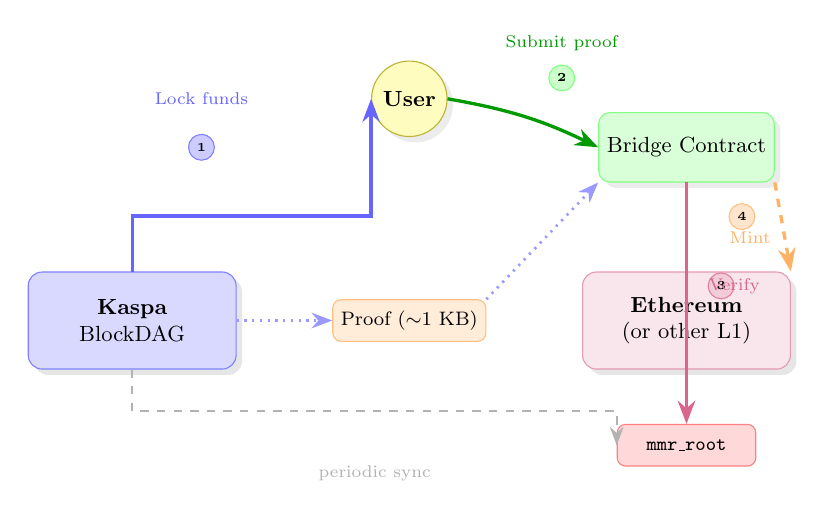
\begin{tikzpicture}[
    chain/.style={rectangle, draw, rounded corners=5pt, minimum width=3cm, minimum height=1.4cm, align=center, font=\small, drop shadow={opacity=0.2}},
    contract/.style={rectangle, draw, rounded corners=4pt, minimum width=2.4cm, minimum height=1cm, align=center, font=\small, drop shadow={opacity=0.15}},
    user/.style={circle, draw=yellow!70!black, fill=yellow!25, minimum size=1cm, font=\small\bfseries, drop shadow={opacity=0.15}},
    databox/.style={rectangle, draw, rounded corners=3pt, font=\footnotesize, minimum width=2cm, align=center, minimum height=0.6cm},
    arrow/.style={->, >=Stealth, thick},
    note/.style={font=\scriptsize},
    scale=0.88, transform shape
]
    % Left side: Kaspa (blue theme)
    \node[chain, fill=blue!15, draw=blue!50] (kaspa) at (0,0) {\textbf{Kaspa}\\BlockDAG};
    
    % Right side: Ethereum (purple theme)
    \node[chain, fill=purple!10, draw=purple!40] (eth) at (8,0) {\textbf{Ethereum}\\(or other L1)};
    \node[contract, fill=green!15, draw=green!50] (bridge) at (8,2.5) {Bridge Contract};
    \node[databox, fill=red!15, draw=red!50, font=\footnotesize\ttfamily] (mmr) at (8,-1.8) {mmr\_root};
    
    % Center: User and Proof
    \node[user] (user) at (4,3.2) {User};
    \node[databox, fill=orange!15, draw=orange!50] (proof) at (4,0) {Proof ($\sim$1 KB)};
    
    % Flow arrows with numbered labels in circles
    \draw[arrow, blue!60, line width=1.2pt] (kaspa.north) -- ++(0,0.8) -| (user.west);
    \node[circle, fill=blue!20, draw=blue!50, font=\tiny\bfseries, inner sep=2pt] at (1,2.5) {1};
    \node[note, text=blue!60] at (1,3.2) {Lock funds};
    
    \draw[arrow, green!60!black, line width=1.2pt] (user.east) to[bend left=8] (bridge.west);
    \node[circle, fill=green!20, draw=green!50, font=\tiny\bfseries, inner sep=2pt] at (6.2,3.5) {2};
    \node[note, text=green!60!black] at (6.2,4) {Submit proof};
    
    \draw[arrow, purple!60, line width=1.2pt] (bridge.south) -- (mmr.north);
    \node[circle, fill=purple!20, draw=purple!50, font=\tiny\bfseries, inner sep=2pt] at (8.5,0.5) {3};
    \node[note, text=purple!60, right] at (8.2,0.5) {Verify};
    
    \draw[arrow, dashed, orange!60, line width=1.2pt] (bridge.south east) -- (eth.north east);
    \node[circle, fill=orange!20, draw=orange!50, font=\tiny\bfseries, inner sep=2pt] at (8.8,1.5) {4};
    \node[note, text=orange!60, right] at (8.5,1.2) {Mint};
    
    % MMR sync (background)
    \draw[arrow, dashed, gray!60] (kaspa.south) -- ++(0,-0.6) -| (mmr.west);
    \node[note, text=gray!60] at (3.5,-2.2) {periodic sync};
    
    % Proof generation flow
    \draw[arrow, dotted, blue!40, line width=1pt] (kaspa.east) -- (proof.west);
    \draw[arrow, dotted, blue!40, line width=1pt] (proof.north east) -- (bridge.south west);
\end{tikzpicture}
\caption{Trustless bridge architecture using MMR proofs. The bridge contract stores only the latest \code{mmr\_root} and verifies inclusion proofs on-chain with $\sim$30 hash operations.}
\label{fig:bridge}
\end{figure}

One primary driver for this feature is to facilitate L2 rollups and cross-chain bridges. With our scheme, an Ethereum contract can store just a single 32-byte \code{mmr\_root} and for each verification, accept a proof and only do $\bigO(\log N)$ hashing.

Furthermore, MMR proofs support batch verification optimization. Multiple transactions can share parts of the proof path, and the peaks list and top-level bagging is common across all proofs. This drastically reduces the risk of bridges---which, as noted by Chainalysis~\cite{chainalysis2022}, have been a major source of hacks when relying on trusted parties.

\textbf{Quantitative Gas Comparison for Cross-Chain Verification:}
\begin{table}[htbp]
\centering
\caption{On-Chain Verification Cost Comparison (Ethereum)}
\label{tab:gas-comparison}
\begin{tabular}{@{}lrrr@{}}
\toprule
\textbf{Proof Depth} & \textbf{KIP-15 Gas} & \textbf{MMR Gas} & \textbf{Feasibility} \\
\midrule
100 blocks & 192,000 & $\sim$15,000 & Both OK \\
1,000 blocks & 1,920,000 & $\sim$21,000 & KIP-15 borderline \\
10,000 blocks & 19,200,000 & $\sim$27,000 & KIP-15 fails \\
100,000 blocks & 192,000,000 & $\sim$35,000 & KIP-15 impossible \\
1,000,000 blocks & 1,920,000,000 & $\sim$42,000 & KIP-15 impossible \\
\bottomrule
\end{tabular}
\end{table}

At 100,000 blocks depth ($\sim$2.8 hours at 10 BPS), KIP-15 exceeds the block gas limit by $6\times$, while MMR verification costs less than $0.1\%$ of the block gas limit.

\subsection{Light Clients and Fast Synchronization}

For Kaspa's own ecosystem, having cryptographic receipts means:
\begin{itemize}
    \item \textbf{Simple Payment Verification (SPV):} A client only needs to track the chain of \code{mmr\_root} in headers and for any transaction of interest, get a proof from a peer and verify it
    \item \textbf{Checkpoint Jumping:} A new node can perform randomized checks against the tip's MMR root
    \item \textbf{Parallelized Download:} Blocks can be downloaded out-of-order and verified in parallel
    \item \textbf{On-demand Historical Retrieval:} Pruned nodes can fetch old data with verifiable proofs
\end{itemize}

\textbf{Skip Verification Strategies:} With an MMR, a node can employ several advanced sync techniques:

\begin{enumerate}
    \item \textbf{Checkpoint Jump:} The node accepts a recent \code{mmr\_root} from a trusted checkpoint or the network. It then downloads blocks in bulk (from any source, even untrusted peers) and verifies each block's \code{order\_root} against its header and then verifies that block's inclusion in the MMR. If any block's data was tampered with, its \code{order\_root} would not match, or its leaf proof would fail. The node can download blocks in parallel and check them in any order---the final \code{mmr\_root} ties them all together.
    
    \item \textbf{Sampling for Security:} If a node doesn't fully trust a given source, it can do random sampling. For example, obtain all block headers from the network (relatively light, just a few GB), thus obtaining the final \code{mmr\_root}. Then download actual transactions for say 1 out of each 100 blocks (randomly chosen), verify those blocks' \code{order\_root}s and MMR proofs. If all samples check out, it has high confidence the history is genuine. This drastically reduces work---checking 1\% of the blocks rather than 100\%.
    
    \item \textbf{Parallel Block Verification:} Even for full verification, ``integrity verification'' can be decoupled from UTXO validation. Multiple threads can verify each block's inclusion independently, sharing the final \code{mmr\_root} as a common reference.
\end{enumerate}

\subsection{Data Availability and Disaster Recovery}

A subtle benefit of having an on-chain history commitment is in data availability and recovery. If historical blocks become unavailable (many nodes pruned and only few archives remain), one might worry about losing that data. With our scheme, as long as the \code{mmr\_root} is known, anyone who eventually finds or reconstructs the block can prove its correctness.

\textbf{Recovery Process:}
\begin{enumerate}
    \item Retrieve recent block headers from peers (which give the recent \code{mmr\_root})
    \item Start from the last trusted checkpoint (e.g., stored MMR state at pruning point)
    \item For each needed block, fetch from any source (could be a torrent, centralized archive, etc.)
    \item Verify block's \code{order\_root} and then verify its inclusion via MMR proof to the known latest root
    \item If all checks pass, safely insert the block into local history
\end{enumerate}

This process ensures that no malicious or corrupted data sneaks in during recovery. The combination of the on-chain commitment and the proofs turns the blockchain history into a \emph{self-verifiable log}---any single block's wrong data breaks the root instantly, strengthening security for archival data.

\subsection{Auditing and Data Availability}

Because the MMR ensures that any omitted or altered transaction would change the root, it provides a solid foundation for audit tools. An auditor could store just the MMR root of each day's tip and later verify any claimed transaction set against it.

%==============================================================================
% SECTION 7: OVERHEAD ANALYSIS
%==============================================================================
\section{Overhead Analysis}
\label{sec:overhead}

\subsection{Bandwidth Overhead}

\begin{table}[htbp]
\centering
\caption{Bandwidth Overhead at 10 BPS}
\label{tab:bandwidth}
\begin{tabular}{@{}lr@{}}
\toprule
\textbf{Metric} & \textbf{Value} \\
\midrule
Additional header bytes & 40 bytes/block \\
Bandwidth at 10 BPS & 400 bytes/sec \\
Daily overhead & $\sim$34.6 MB \\
Yearly overhead & $\sim$12.6 GB \\
Relative to block data ($\sim$50 KB/block) & $<0.1\%$ \\
\bottomrule
\end{tabular}
\end{table}

\subsection{Storage Overhead}

\begin{figure}[htbp]
\centering
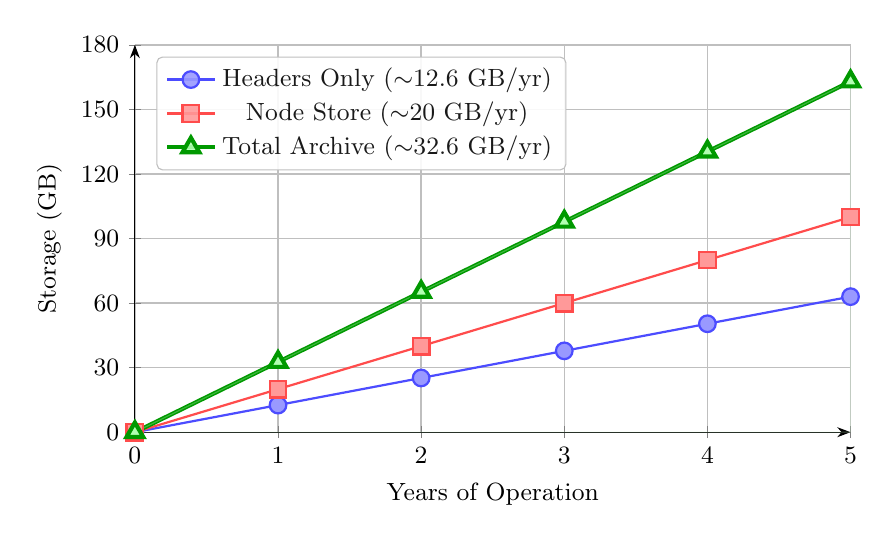
\begin{tikzpicture}
\begin{axis}[
    xlabel={Years of Operation},
    ylabel={Storage (GB)},
    legend pos=north west,
    legend style={font=\small, rounded corners=2pt, fill=white, fill opacity=0.9, draw=gray!50},
    grid=both,
    grid style={line width=0.3pt, draw=gray!30},
    major grid style={line width=0.5pt, draw=gray!50},
    width=0.88\textwidth,
    height=6.5cm,
    xmin=0, xmax=5,
    ymin=0, ymax=180,
    xtick={0,1,2,3,4,5},
    ytick={0,30,60,90,120,150,180},
    tick label style={font=\small},
    label style={font=\small},
    axis lines=left,
    axis line style={->, >=Stealth},
]
\addplot[blue!70, thick, mark=*, mark size=3pt, mark options={fill=blue!40}] coordinates {
    (0,0) (1,12.6) (2,25.2) (3,37.8) (4,50.4) (5,63)
};
\addplot[red!70, thick, mark=square*, mark size=3pt, mark options={fill=red!40}] coordinates {
    (0,0) (1,20) (2,40) (3,60) (4,80) (5,100)
};
\addplot[green!60!black, thick, mark=triangle*, mark size=3.5pt, mark options={fill=green!30}, line width=1.5pt] coordinates {
    (0,0) (1,32.6) (2,65.2) (3,97.8) (4,130.4) (5,163)
};

% Add fill area for total
\addplot[green!20, forget plot, opacity=0.3] coordinates {
    (0,0) (1,32.6) (2,65.2) (3,97.8) (4,130.4) (5,163) (5,0) (0,0)
} \closedcycle;

\legend{Headers Only ($\sim$12.6 GB/yr), Node Store ($\sim$20 GB/yr), Total Archive ($\sim$32.6 GB/yr)}
\end{axis}
\end{tikzpicture}
\caption{Storage growth over time at 10 BPS. Headers grow at $\sim$12.6 GB/year; optional node store for proof generation adds $\sim$20 GB/year. Even after 5 years, total storage remains under 165 GB---manageable for modern hardware.}
\label{fig:storage}
\end{figure}

\subsection{Computation Overhead}

Per-block hashing operations:
\begin{itemize}
    \item Merkle root computation: $\bigO(\log m)$ hashes (same as before)
    \item MMR update: Average $<2$ hashes, worst case $\sim\log N$ hashes
    \item Total: Negligible compared to PoW and signature verification
\end{itemize}

The trade-off is extremely favorable: for a modest storage and negligible performance cost, Kaspa gains a built-in universal proof system for its transaction history.

%==============================================================================
% SECTION 8: COMPARISON
%==============================================================================
\section{Comparison with Alternative Approaches}
\label{sec:comparison}

In this section, we provide a detailed comparison between our MMR-based unified approach and the two Kaspa Improvement Proposals that inspired it: KIP-6 (Proof of Chain Membership) and KIP-15 (Canonical Transaction Ordering and Sequencing Commitment). Understanding the design philosophy, strengths, and limitations of each approach illuminates why our unified solution represents an optimal path forward.

\subsection{KIP-15: Linear Sequencing Commitment}

\subsubsection{Design Philosophy and Mechanism}

KIP-15, authored by Mike Zak and Ro Ma~\cite{kip15}, addresses a fundamental need for Layer-2 networks: the ability to trustlessly verify the \emph{order} of transaction acceptance on L1. The proposal recognizes that L2 networks rely on Kaspa for both consensus and data availability, where ``the ordering of transaction acceptance in L1 has to be the ordering of transaction execution on L2.''

The core mechanism introduces a new header field called \code{SequencingCommitment}, calculated as:
\begin{equation}
\text{SC}_B = H(\text{SC}_{P_{sel}(B)} \parallel \text{AcceptedIDMerkleRoot}_B)
\end{equation}
where $P_{sel}(B)$ is the selected parent of block $B$.

\begin{figure}[htbp]
\centering
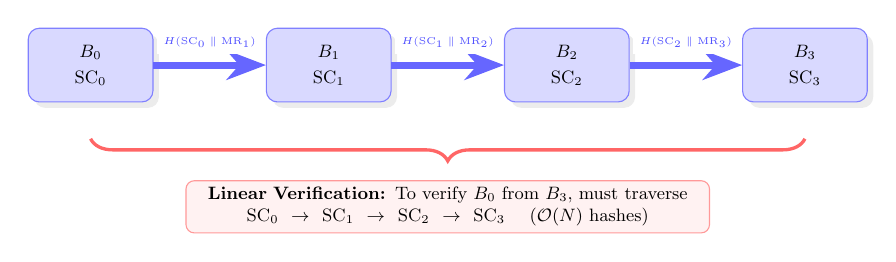
\begin{tikzpicture}[
    block/.style={rectangle, draw=blue!50, fill=blue!15, minimum width=2.2cm, minimum height=1.3cm, rounded corners=4pt, font=\small, align=center, drop shadow={opacity=0.15}},
    arrow/.style={->, >=Stealth, thick},
    scale=0.72, transform shape
]
    % Block chain
    \node[block] (b0) at (0,0) {$B_0$\\[2pt]$\text{SC}_0$};
    \node[block] (b1) at (4.2,0) {$B_1$\\[2pt]$\text{SC}_1$};
    \node[block] (b2) at (8.4,0) {$B_2$\\[2pt]$\text{SC}_2$};
    \node[block] (b3) at (12.6,0) {$B_3$\\[2pt]$\text{SC}_3$};
    
    % Chain links with hash formulas
    \draw[arrow, line width=2.5pt, blue!60] (b0) -- (b1);
    \node[fill=white, font=\tiny, text=blue!70] at (2.1,0.4) {$H(\text{SC}_0 \parallel \text{MR}_1)$};
    
    \draw[arrow, line width=2.5pt, blue!60] (b1) -- (b2);
    \node[fill=white, font=\tiny, text=blue!70] at (6.3,0.4) {$H(\text{SC}_1 \parallel \text{MR}_2)$};
    
    \draw[arrow, line width=2.5pt, blue!60] (b2) -- (b3);
    \node[fill=white, font=\tiny, text=blue!70] at (10.5,0.4) {$H(\text{SC}_2 \parallel \text{MR}_3)$};
    
    % Verification path indicator
    \draw[decorate, decoration={brace, amplitude=8pt, mirror}, red!60, line width=1.2pt] (0,-1.3) -- (12.6,-1.3);
    
    % Explanation box
    \node[draw=red!40, fill=red!5, rounded corners=3pt, font=\small, align=center, text width=9cm] at (6.3,-2.5) {
        \textbf{Linear Verification:} To verify $B_0$ from $B_3$, must traverse\\
        $\text{SC}_0 \to \text{SC}_1 \to \text{SC}_2 \to \text{SC}_3$ \quad ($\bigO(N)$ hashes)
    };
\end{tikzpicture}
\caption{KIP-15 Linear Sequencing Commitment. Each block's SC depends on its parent's SC, creating a sequential chain. Verification requires traversing all intermediate commitments.}
\label{fig:kip15-chain}
\end{figure}

Additionally, KIP-15 proposes a critical change: the \code{AcceptedIDMerkleRoot} should preserve \emph{canonical order} rather than sorting transactions by hash. The original hash-sorting was an optimization for exclusion proofs, but as KIP-15 notes: ``there is currently no application on top of Kaspa using the above feature.''

\subsubsection{Strengths}

\begin{enumerate}
    \item \textbf{Simplicity:} One additional hash per block; minimal implementation complexity
    \item \textbf{Strong Ordering Guarantee:} The chain of commitments cryptographically binds the exact sequence of all accepted transactions
    \item \textbf{ATAN Support:} Enables Accepted Transactions Archival Nodes to bootstrap from untrusted sources with verification
    \item \textbf{Low Header Overhead:} Replaces existing field rather than adding new ones (net change: 0 bytes)
\end{enumerate}

\subsubsection{Limitations}

\begin{enumerate}
    \item \textbf{Linear Verification Complexity:} To verify that a transaction in block $N$ is part of the history up to block $M$, one must compute or provide all $M-N$ intermediate commitments. As stated in the KIP: ``downloading and validating a cryptographic proof testifying to the above'' requires processing the entire selected parent chain.
    
    \item \textbf{No Skip-Ahead Capability:} The sequential dependency prevents any form of random access or parallel verification.
    
    \item \textbf{Impractical for Bridges:} On-chain verification (e.g., in an Ethereum smart contract) of a proof spanning 100,000 blocks would require $\sim$100,000 hash operations---exceeding any reasonable gas limit by orders of magnitude.
    
    \item \textbf{No Independence from KIP-6:} KIP-15 alone does not provide efficient proofs of chain membership; the document's ATAN design assumes full header availability.
\end{enumerate}

\subsection{KIP-6: Proof of Chain Membership (PoChM)}

\subsubsection{Design Philosophy and Mechanism}

KIP-6, authored by Shai Wyborski~\cite{kip6}, addresses a complementary problem: providing cryptographically verifiable proofs that a transaction was included in the blockchain, especially after pruning has occurred. The proposal recognizes that ``the pruning mechanism makes it impossible to prove that a transaction was included in the ledger after it has been pruned'' and that relying on centralized archival nodes ``is not a sustainable solution.''

KIP-6 introduces the concept of \textbf{Posterity Headers}---selected chain block headers sampled at regular intervals (currently every 24 hours, coinciding with pruning blocks) and stored indefinitely. The core mechanism adds a \textbf{PoChM Merkle Root (PMR)} to each header:

\begin{definition}[PMR Construction (KIP-6)]
Let $k$ be the least integer such that $\text{parent}(B, 2^k) \in \text{Past}(\text{next\_posterity}(B))$. Then PMR is the root of the Merkle tree containing the headers $\text{parent}(B, 2^i)$ for $i = 0, \ldots, k-1$.
\end{definition}

This creates a skip-list-like structure where each block commits to ancestors at exponentially increasing distances ($2^0, 2^1, 2^2, \ldots$).

\begin{figure}[htbp]
\centering
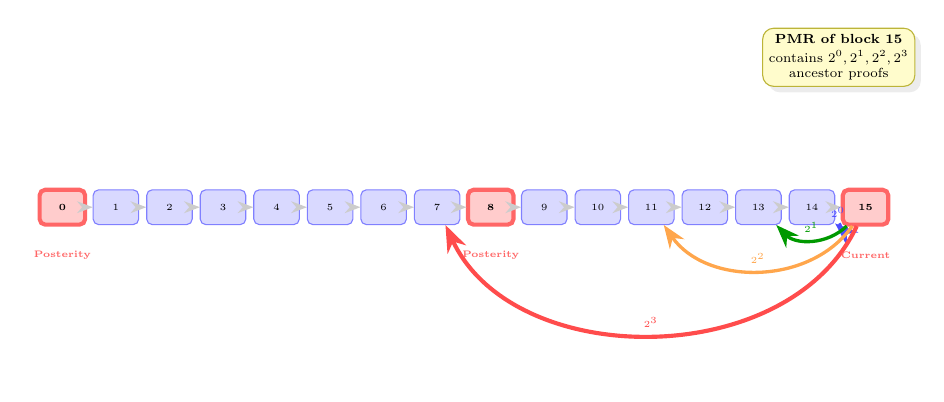
\begin{tikzpicture}[
    block/.style={rectangle, draw=blue!50, fill=blue!15, minimum width=0.85cm, minimum height=0.65cm, font=\tiny, rounded corners=2pt},
    posterity/.style={rectangle, draw=red!60, fill=red!20, minimum width=0.85cm, minimum height=0.65cm, font=\tiny\bfseries, line width=1.5pt, rounded corners=2pt},
    arrow/.style={->, >=Stealth},
    skip/.style={->, >=Stealth, thick},
    scale=0.68, transform shape
]
    % Blocks
    \foreach \i in {0,...,15} {
        \pgfmathtruncatemacro{\mod}{\i == 0 || \i == 8 || \i == 15}
        \ifnum\mod=1
            \node[posterity] (b\i) at (\i*1.0,0) {\i};
        \else
            \node[block] (b\i) at (\i*1.0,0) {\i};
        \fi
    }
    
    % Normal chain (subtle)
    \foreach \i in {1,...,15} {
        \pgfmathtruncatemacro{\prev}{\i-1}
        \draw[arrow, gray!40, line width=0.6pt] (b\prev) -- (b\i);
    }
    
    % Skip pointers from block 15 with gradient colors
    \draw[skip, blue!70, line width=1.2pt] (b15) to[bend left=35] node[above, font=\tiny\bfseries, text=blue!70] {$2^0$} (b14);
    \draw[skip, green!60!black, line width=1.2pt] (b15) to[bend left=45] node[above, font=\tiny\bfseries, text=green!60!black] {$2^1$} (b13);
    \draw[skip, orange!70, line width=1.2pt] (b15) to[bend left=55] node[above, font=\tiny\bfseries, text=orange!70] {$2^2$} (b11);
    \draw[skip, red!70, line width=1.5pt] (b15) to[bend left=65] node[above, font=\tiny\bfseries, text=red!70] {$2^3$} (b7);
    
    % PMR annotation box
    \node[draw=yellow!70!black, rounded corners=4pt, fill=yellow!20, font=\scriptsize, align=center, drop shadow={opacity=0.15}] at (14.5,2.8) {
        \textbf{PMR of block 15}\\[2pt]
        contains $2^0, 2^1, 2^2, 2^3$\\
        ancestor proofs
    };
    
    % Posterity block labels
    \node[font=\tiny\bfseries, text=red!60] at (0,-0.9) {Posterity};
    \node[font=\tiny\bfseries, text=red!60] at (8,-0.9) {Posterity};
    \node[font=\tiny\bfseries, text=red!60] at (15,-0.9) {Current};
\end{tikzpicture}
\caption{KIP-6 PoChM Structure with exponential skip pointers ($2^i$). Each block's PMR contains Merkle proofs of ancestors at distances $2^0, 2^1, 2^2, \ldots$ The proof path uses binary decomposition of the distance.}
\label{fig:kip6-skiplist}
\end{figure}

\subsubsection{Proof Construction Algorithm}

The PoChM generation algorithm (from KIP-6) uses binary decomposition:
\begin{enumerate}
    \item Let $C = \text{posterity}(B)$ and $d = \text{posterity\_depth}(B)$
    \item While $d > 0$:
    \begin{itemize}
        \item Let $i = \lfloor \log_2(d) \rfloor$
        \item Append $\text{PMR}(C, i)$ to proof
        \item $d \gets d - 2^i$; $C \gets \text{parent}(C, 2^i)$
    \end{itemize}
\end{enumerate}

This yields proof complexity of $\bigO(\log N \cdot \log \log N)$ where $N$ is the number of chain blocks between posterity headers.

\subsubsection{Strengths}

\begin{enumerate}
    \item \textbf{Logarithmic Proofs:} Proof size is $\bigO(\log N \cdot \log \log N)$, approximately 9 KB worst case
    \item \textbf{Minimal Header Overhead:} Only 32 bytes (one hash) added per header
    \item \textbf{Efficient Validation:} 33 hashes per block for chain blocks
    \item \textbf{Pruning Compatible:} Proofs can be generated before pruning and verified indefinitely
    \item \textbf{Elegant Binary Decomposition:} Mathematically principled approach leveraging number-theoretic structure
\end{enumerate}

\subsubsection{Limitations}

\begin{enumerate}
    \item \textbf{Does Not Commit Transaction Order:} KIP-6 provides proofs that a block was in the selected chain, but not the canonical ordering of transactions. As stated: ``a PoChM for B is also a PoChM for any chain block C $\in$ Future(B) $\cap$ Past(posterity(B))''---the proof is about chain membership, not transaction sequence.
    
    \item \textbf{Requires Separate Structure for Ordering:} To prove both chain membership \emph{and} transaction order, KIP-6 must be combined with KIP-15 or similar, resulting in two parallel commitment structures.
    
    \item \textbf{Posterity Header Dependency:} The scheme depends on posterity headers (currently 24-hour intervals). This introduces latency: a PoChM cannot be generated until the next posterity header exists.
    
    \item \textbf{Complex Proof Structure:} The $\log \log N$ factor comes from Merkle proofs within the PMR tree. While asymptotically minor, it adds implementation complexity.
    
    \item \textbf{Not Optimized for Batch Proofs:} Multiple independent proofs don't naturally share structure.
\end{enumerate}

\subsection{Comparative Analysis: Deep Insights}

\subsubsection{The Fundamental Tension}

KIP-15 and KIP-6 represent two orthogonal responses to the same underlying challenge: how to provide verifiable historical information in a pruning blockchain.

\begin{itemize}
    \item \textbf{KIP-15} prioritizes \emph{ordering integrity}---ensuring the canonical sequence of transactions is cryptographically committed and verifiable.
    \item \textbf{KIP-6} prioritizes \emph{proof efficiency}---ensuring historical claims can be verified with logarithmic-sized proofs.
\end{itemize}

Neither alone solves the complete problem. A Layer-2 rollup or cross-chain bridge needs \emph{both}: proof that a transaction was accepted (KIP-6's domain) \emph{and} proof of its position in the global order (KIP-15's domain).

\subsubsection{The Architectural Incompatibility}

Implementing KIP-15 and KIP-6 together creates architectural friction:

\begin{enumerate}
    \item \textbf{Dual Commitment Overhead:} Two separate header fields, two separate validation paths, two separate proof structures.
    
    \item \textbf{Proof Composition Complexity:} A complete ``transaction receipt'' would require:
    \begin{itemize}
        \item A PoChM (from KIP-6) proving block chain membership
        \item A Merkle proof for transaction within block's ATMR
        \item A chain of SequencingCommitments (from KIP-15) if ordering matters
    \end{itemize}
    The third component reintroduces linear complexity, negating KIP-6's benefits for order-sensitive applications.
    
    \item \textbf{Conceptual Overlap Without Synergy:} Both proposals touch block headers and validation rules, but don't reinforce each other's proofs.
\end{enumerate}

\subsubsection{Why MMR is the Natural Synthesis}

Our MMR-based approach resolves this tension through \emph{structural unification}:

\begin{enumerate}
    \item \textbf{Inherent Ordering via Leaf Sequence:} Each MMR leaf corresponds to a specific position in the selected chain. The leaf's index \emph{is} the block's position in the canonical sequence. Transaction order is encoded by: (a) the block's MMR leaf index, and (b) the transaction's position within the block's $\OrderRoot$.
    
    \item \textbf{Logarithmic Proofs for Both Membership and Order:} A single MMR proof demonstrates both that a block was in the chain \emph{and} its exact position. No linear traversal is needed.
    
    \item \textbf{Unified Header Field:} The \code{order\_root} commits to transaction ordering (KIP-15's goal), while the \code{mmr\_root} enables efficient proofs (KIP-6's goal). These naturally compose rather than compete.
\end{enumerate}

\begin{table}[htbp]
\centering
\caption{Detailed Feature Comparison: KIP-6, KIP-15, and MMR-Based Approach}
\label{tab:detailed-comparison}
\small
\begin{tabular}{@{}p{3.2cm}p{3.5cm}p{3.5cm}p{3.8cm}@{}}
\toprule
\textbf{Aspect} & \textbf{KIP-15} & \textbf{KIP-6} & \textbf{MMR (Ours)} \\
\midrule
\multicolumn{4}{l}{\textit{Core Functionality}} \\
\midrule
Commits TX Order & \cmark{} (chain hash) & \xmark{} & \cmark{} (via $\OrderRoot$) \\
Efficient Inclusion Proof & \xmark{} ($\bigO(N)$) & \cmark{} ($\bigO(\log N \log\log N)$) & \cmark{} ($\bigO(\log N)$) \\
Proves Position in History & \cmark{} (implicitly) & \xmark{} (block only) & \cmark{} (explicitly) \\
\midrule
\multicolumn{4}{l}{\textit{Proof Characteristics}} \\
\midrule
Proof size (depth $D$) & $\bigO(D) \times 32$B & $\bigO(\log D \log\log D) \times 32$B & $\bigO(\log D) \times 32$B \\
Proof at 100K blocks & $\sim$3.2 MB & $\sim$9 KB & $\sim$1 KB \\
Proof at 1M blocks & $\sim$32 MB & $\sim$11 KB & $\sim$1.1 KB \\
On-chain verifiable & \xmark{} (exceeds gas) & \cmark{} & \cmark{} \\
\midrule
\multicolumn{4}{l}{\textit{Implementation}} \\
\midrule
Header overhead & 0 bytes (replace) & +32 bytes & +40 bytes (net) \\
Hashes per block & 1 & $\sim$33 (chain blocks) & $\sim$5--10 (average) \\
External dependency & None & Posterity headers & None \\
\midrule
\multicolumn{4}{l}{\textit{Use Case Support}} \\
\midrule
ATAN sync (ordering) & \cmark{} (linear) & \xmark{} & \cmark{} (logarithmic) \\
L2 rollup proofs & \xmark{} (too large) & Partial (no order) & \cmark{} \\
Cross-chain bridge & \xmark{} & \cmark{} & \cmark{} \\
Light client SPV & \xmark{} & \cmark{} & \cmark{} \\
Batch proof optimization & \xmark{} & Limited & \cmark{} (shared peaks) \\
\bottomrule
\end{tabular}
\end{table}

\subsubsection{Quantitative Analysis: Gas Cost Comparison}

For cross-chain bridge applications, on-chain verification cost is critical. We compare the gas requirements for verifying a transaction that occurred $D$ blocks ago:

\begin{figure}[htbp]
\centering
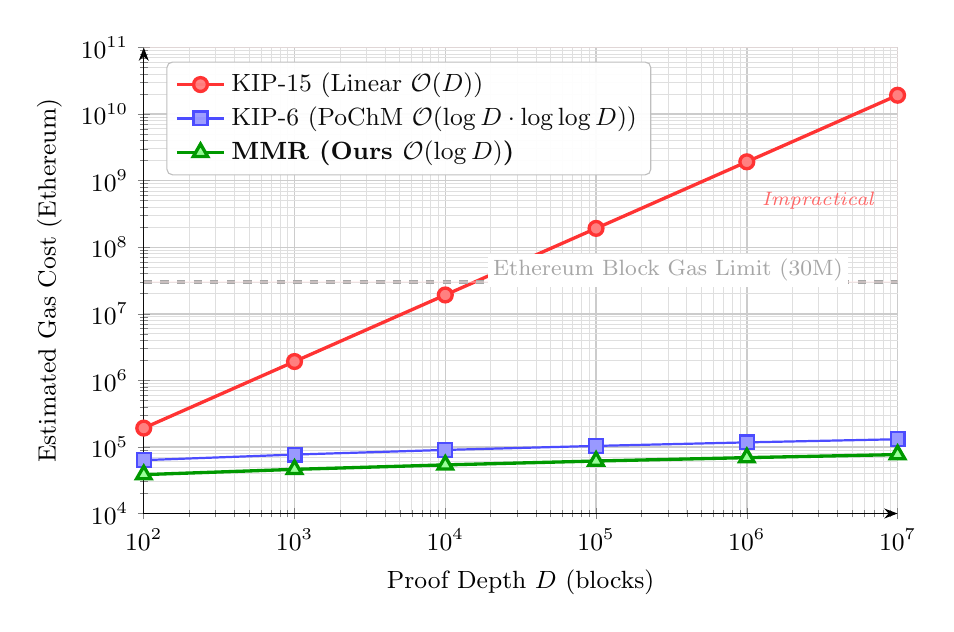
\begin{tikzpicture}
\begin{axis}[
    xlabel={Proof Depth $D$ (blocks)},
    ylabel={Estimated Gas Cost (Ethereum)},
    ymode=log,
    xmode=log,
    log basis y={10},
    log basis x={10},
    legend pos=north west,
    legend style={font=\small, rounded corners=2pt, fill=white, fill opacity=0.95, draw=gray!50, cells={anchor=west}},
    grid=both,
    grid style={line width=0.3pt, draw=gray!25},
    major grid style={line width=0.5pt, draw=gray!40},
    width=0.92\textwidth,
    height=7.5cm,
    xmin=100, xmax=10000000,
    ymin=10000, ymax=100000000000,
    tick label style={font=\small},
    label style={font=\small},
    axis lines=left,
    axis line style={->, >=Stealth},
]
% KIP-15: Linear (red, impractical)
\addplot[red!80, very thick, mark=*, mark size=2.5pt, mark options={fill=red!50}] coordinates {
    (100, 192000) (1000, 1920000) (10000, 19200000) (100000, 192000000) (1000000, 1920000000) (10000000, 19200000000)
};
% KIP-6: O(log D * log log D)
\addplot[blue!70, thick, mark=square*, mark size=2.5pt, mark options={fill=blue!40}] coordinates {
    (100, 63360) (1000, 76800) (10000, 90240) (100000, 103680) (1000000, 117120) (10000000, 130560)
};
% MMR: O(log D) - best
\addplot[green!60!black, very thick, mark=triangle*, mark size=3pt, mark options={fill=green!40}] coordinates {
    (100, 38400) (1000, 46080) (10000, 53760) (100000, 61440) (1000000, 69120) (10000000, 76800)
};

% Ethereum block gas limit reference line
\addplot[dashed, gray!70, line width=1.5pt] coordinates {(100, 30000000) (10000000, 30000000)};

% Fill area above gas limit (impractical zone)
\addplot[red!10, forget plot, opacity=0.4] coordinates {
    (100, 30000000) (10000000, 30000000) (10000000, 100000000000) (100, 100000000000)
} \closedcycle;

% Gas limit label
\node[font=\footnotesize, text=gray!70, fill=white, inner sep=2pt] at (axis cs:300000, 45000000) {Ethereum Block Gas Limit (30M)};

% Annotation for impractical zone
\node[font=\scriptsize, text=red!60, rotate=0] at (axis cs:3000000, 500000000) {\textit{Impractical}};

\legend{KIP-15 (Linear $\bigO(D)$), KIP-6 (PoChM $\bigO(\log D \cdot \log\log D)$), \textbf{MMR (Ours $\bigO(\log D)$)}}
\end{axis}
\end{tikzpicture}
\caption{On-chain verification gas cost comparison. KIP-15's linear growth makes it impractical beyond $\sim$15,000 blocks (crosses gas limit). Both KIP-6 and MMR remain feasible at any depth, with MMR offering $\sim$40\% lower costs due to simpler proof structure.}
\label{fig:gas-deep-comparison}
\end{figure}

\begin{proposition}[Gas Cost Bounds]
For a proof of depth $D$ blocks:
\begin{align}
\text{Gas}_{\text{KIP-15}} &= 1920 \times D \\
\text{Gas}_{\text{KIP-6}} &\approx 1920 \times (2 \log_2 D \times \lceil \log_2 \log_2 D \rceil + 1) \\
\text{Gas}_{\text{MMR}} &\approx 1920 \times (\log_2 D + k)
\end{align}
where $k$ is the number of peaks ($k \leq \log_2 D$, typically much smaller).
\end{proposition}

At $D = 100,000$ blocks ($\sim$2.8 hours at 10 BPS):
\begin{itemize}
    \item KIP-15: 192 million gas (exceeds block limit by 6$\times$)
    \item KIP-6: $\sim$104,000 gas (feasible)
    \item MMR: $\sim$61,000 gas (feasible, 41\% lower than KIP-6)
\end{itemize}

\subsubsection{Architectural Elegance: The MMR Advantage}

Beyond quantitative metrics, the MMR approach offers qualitative advantages:

\begin{enumerate}
    \item \textbf{Conceptual Simplicity:} One data structure serves both purposes. Developers need only understand MMRs, not the interaction between skip-lists (KIP-6) and hash chains (KIP-15).
    
    \item \textbf{Proof Composability:} Multiple transactions from different blocks can share the same peak list in their proofs, enabling efficient batch verification.
    
    \item \textbf{No Posterity Dependency:} Unlike KIP-6, MMR proofs can be generated immediately after block confirmation---no waiting for posterity header creation.
    
    \item \textbf{Natural Append-Only Semantics:} MMR's structure mirrors the blockchain's append-only nature, making reorg handling straightforward.
    
    \item \textbf{Industry Precedent:} MMRs are battle-tested in Grin, Beam, and Nervos, providing implementation guidance and security confidence.
\end{enumerate}

\subsection{Summary: Why Unification Matters}

The fundamental insight driving our proposal is that \emph{ordering commitment and efficient proofs are not independent problems}---they are two facets of the same challenge: providing verifiable historical information in a resource-constrained environment.

\begin{quote}
\textit{KIP-15 asks: ``How do we commit to the order?''\\
KIP-6 asks: ``How do we prove membership efficiently?''\\
MMR answers both: ``By embedding the order in an efficient accumulator.''}
\end{quote}

Implementing KIP-6 and KIP-15 separately would require:
\begin{itemize}
    \item Two consensus changes
    \item Two header fields
    \item Two validation codepaths
    \item Two proof formats
    \item Complex interaction semantics
\end{itemize}

Our MMR-based design delivers equivalent (and superior) functionality through a single, unified mechanism---embodying the engineering principle that the best solution is often one that \emph{eliminates} the distinction between seemingly separate problems.

\begin{table}[htbp]
\centering
\caption{Summary Comparison of Transaction Commitment Approaches}
\label{tab:summary-comparison}
\small
\begin{tabular}{@{}p{3.5cm}ccc@{}}
\toprule
\textbf{Capability} & \textbf{KIP-15} & \textbf{KIP-6} & \textbf{MMR (Ours)} \\
\midrule
Commits to global order & \cmark{} & \xmark{} & \cmark{} \\
Supports $\bigO(\log n)$ proofs & \xmark{} & \cmark{} & \cmark{} \\
Jump/skip verification & \xmark{} & \cmark{} & \cmark{} \\
L2-friendly (gas cost) & Poor & Good & Excellent \\
Additional data structures & None & Complex & None \\
Implementation complexity & Low & Medium/High & Medium \\
\bottomrule
\end{tabular}
\end{table}

This aligns with broader industry trends: Ethereum's Verkle trees for state, Bitcoin's work on Utreexo, and various succinct proof protocols all strive to make blockchain data more accessible without full trust or full nodes. Kaspa's adoption of MMR commitments would be among the first in a live L1 blockchain, and we believe it will greatly enhance the ecosystem's capabilities.

%==============================================================================
% SECTION 9: IMPLEMENTATION
%==============================================================================
\section{Implementation and Deployment}
\label{sec:implementation}

\subsection{Activation via Network Upgrade}

Because this change affects the consensus (block header and validation), it must be introduced via a \textbf{hard fork}. We choose an activation point (e.g., a DAA score threshold or timestamp). Blocks after that must include the new fields and follow the new validation logic.

\subsection{Miner Integration}

Miners need to upgrade their block template generation:
\begin{enumerate}
    \item Compute \code{order\_root} from accepted transactions
    \item Fetch current MMR state from node (peaks and size)
    \item Compute new leaf hash and updated \code{mmr\_root} and \code{mmr\_size}
    \item Populate these in the header, then perform PoW
\end{enumerate}

\subsection{Data Structures and APIs}

New database structures:
\begin{itemize}
    \item \code{mmr\_state\_store}: Block hash $\to$ MMR state (peaks list + size)
    \item \code{mmr\_node\_store}: MMR position $\to$ hash (optional, for proof generation)
\end{itemize}

New RPC endpoints:
\begin{itemize}
    \item \code{GetMmrProof(blockHash, targetBlockHash)}: Returns inclusion proof
    \item \code{VerifyTransactionProof(proof)}: Validates a given proof
\end{itemize}

\subsection{Security Considerations}

\begin{itemize}
    \item \textbf{Collision Resistance:} Domain separation ensures no hash collisions across different contexts
    \item \textbf{Replay Protection:} MMR root is in the block header, so tampering requires re-mining
    \item \textbf{Denial of Service:} Proof verification is fast ($\sim$30 hashes maximum)
    \item \textbf{Reorg Exploit:} Cryptographic hashing prevents same MMR root for different histories
\end{itemize}

%==============================================================================
% SECTION 10: CONCLUSION
%==============================================================================
\section{Conclusion}
\label{sec:conclusion}

We have presented a unified approach to incorporating Sequencing Commitments in Kaspa using a Merkle Mountain Range (MMR) structure, achieving both canonical transaction ordering commitment and efficient logarithmic proofs for transaction inclusion. This design meets the requirements of KIP-15 and KIP-6 simultaneously, simplifying implementation and maintenance.

\subsection{Summary of Results}

Our scheme adds a small overhead (40 bytes per block) to the Kaspa headers, which is negligible relative to block sizes and bandwidth. It modestly increases storage requirements (on the order of tens of GB per year for a full archival node), which is a worthwhile trade for the added functionality. In return, Kaspa gains:

\begin{enumerate}
    \item \textbf{Verifiable Transaction Order:} Every block locks in the exact order of all transactions up to that point. This enhances the determinism and auditability of the ledger.
    
    \item \textbf{Compact Proofs:} Any transaction in history can be proven to a light client or contract with a proof on the order of 0.5--1~KB, regardless of how old it is, enabling cross-chain verification and light clients without trusted servers.
    
    \item \textbf{Support for Decentralized L2:} Rollups on Kaspa can use the L1 as a data availability and ordering layer directly, leveraging the commitment to sequence. L2 state transitions can be verified knowing the order of L1 transactions (no alternative histories to consider).
    
    \item \textbf{Efficient Sync \& Recovery:} Nodes can sync faster and recover from data loss using the MMR commitments to validate bulk data from untrusted sources. This reduces reliance on trusted archives or intensive bootstrap processes, contributing to network resilience and decentralization.
    
    \item \textbf{Self-Authenticating History:} The whole history becomes verifiable against the latest block. Any single block's wrong data breaks the MMR root instantly---analogous to how a Merkle root turns a block's transactions into a verifiable set, now extended to the entire blockchain level.
\end{enumerate}

The unified approach subsumes both KIP-15 (sequencing) and KIP-6 (logarithmic proofs) in a single coherent design, simplifying implementation while delivering enhanced functionality. The proof size remains around 1~KB even for millions of blocks, and on-chain verification requires only $\sim$30 hashes ($\sim$60,000 gas on Ethereum).

\subsection{Future Work}

\begin{itemize}
    \item \textbf{SNARK/STARK Compression:} Potentially reduce proof size to constant using zero-knowledge proofs, enabling even more efficient cross-chain verification
    
    \item \textbf{Multi-proof Aggregation:} Batch verification optimizations for bridge contracts handling many transactions simultaneously
    
    \item \textbf{Cross-chain Applications:} Adapting the scheme for other DAG-based ledgers or even traditional blockchains
    
    \item \textbf{Light Client Protocols:} Building improved light client protocols where light nodes only track headers and use the MMR for occasional proofs to confirm state changes or detect forks---essentially enabling NiPoPoW-like proofs of transactions, not just chain progress
    
    \item \textbf{Transaction Exclusion Proofs:} Ensuring a transaction was not included by a certain point (can be achieved by proving inclusion of a conflicting tx or reaching a certain block without inclusion)
    
    \item \textbf{Security Analysis:} Formal security analysis proving that subverting the log (e.g., including a transaction out of order or forging a history) would require breaking cryptographic hash collision resistance
\end{itemize}

Our approach underscores a general principle: by turning the blockchain (or blockDAG) history into a cryptographically authenticated data structure (a verifiable log), we empower light clients and cross-chain systems to interact with the blockchain trustlessly. As Kaspa continues to push the limits of blockDAG performance, features like this ensure that its security and usability for advanced applications keep pace. We anticipate this will accelerate development of L2 ecosystems around Kaspa and serve as a model for other projects seeking efficient historical proof systems.

%==============================================================================
% REFERENCES
%==============================================================================
\newpage
\begin{thebibliography}{99}

\bibitem{kip15}
Kaspa Improvement Proposal KIP-15: Sequencing Commitments for Transaction Ordering.
\textit{Kaspa Updates to Crescendo and 10BPS}, 2024.
\url{https://kaspa.org/kaspa-updates-to-crescendo-and-10bps/}

\bibitem{kip6}
Kaspa Improvement Proposal KIP-6: Logarithmic Transaction Inclusion Proofs.
\textit{Kaspa Improvement Proposals}, 2023.
\url{https://github.com/kaspanet/kips/blob/master/kip-0006.md}

\bibitem{herodotus}
Herodotus Protocol Documentation: Merkle Mountain Ranges.
\textit{Herodotus Docs}, 2024.
\url{https://docs.herodotus.dev/herodotus-docs/protocol-design/historical-block-hash-accumulator/merkle-mountain-ranges}

\bibitem{ghostdag}
Y. Sompolinsky, S. Wyborski, and A. Zohar,
``Phantom and GhostDAG: A Scalable Generalization of Nakamoto Consensus,''
\textit{Cryptology ePrint Archive}, Report 2018/104, 2021.

\bibitem{nervos}
Nervos Network,
``RFC: Merkle Mountain Range,''
\textit{Nervos RFCs}, 2019.

\bibitem{grin}
Grin Documentation,
``Merkle Mountain Ranges,''
\textit{Grin Wiki}, 2019.

\bibitem{todd2012mmr}
P. Todd,
``Merkle Mountain Ranges,''
\textit{Bitcoin Development Mailing List}, 2012.

\bibitem{kaspa2021}
M. Sompolinsky et al.,
``PHANTOM GHOSTDAG: A Scalable Generalization of Nakamoto Consensus,''
\textit{Proceedings of the 3rd ACM Conference on Advances in Financial Technologies}, 2021.

\bibitem{wood2016}
G. Wood,
``Ethereum: A Secure Decentralised Generalised Transaction Ledger,''
\textit{Ethereum Yellow Paper}, 2016.

\bibitem{nakamoto2008}
S. Nakamoto,
``Bitcoin: A Peer-to-Peer Electronic Cash System,''
2008.

\bibitem{flyclient}
B. Bünz, L. Kiffer, L. Luu, and M. Zamani,
``FlyClient: Super-Light Clients for Cryptocurrencies,''
\textit{IEEE Symposium on Security and Privacy (S\&P)}, 2020.

\bibitem{nipopow}
A. Kiayias, A. Miller, and D. Zindros,
``Non-Interactive Proofs of Proof-of-Work,''
\textit{Financial Cryptography and Data Security}, 2020.

\bibitem{merklebelt}
G. A. Marson, et al.,
``The Merkle Mountain Belt,''
\textit{arXiv preprint arXiv:2511.13582}, 2025.

\bibitem{chainalysis2022}
Chainalysis,
``Crypto Bridge Hacks in 2022: Statistics on Bridge Vulnerabilities,''
\textit{Chainalysis Reports}, 2022.

\end{thebibliography}

\end{document}